\documentclass[11pt]{article}
\title{Meccano pentagons gallery}
\author{https://github.com/heptagons/meccano/penta/gallery}
\date{2023/12/13}

\usepackage{../../meccano}
\usepackage{amssymb}

\begin{document}

\maketitle
\begin{abstract}
We build rigid meccano\meccanoref regular pentagons from sides $3$ to $12$. We restrict all internal strips to remain inside the pentagon's perimeter and don't permit they overlap with others. We follow three steps. 1) We calculate distances between selected strips holes from the regular pentagon perimeter assuming is regular. 2) We run some programs available in this repo to look for rigid clusters of strips which contains the distance. 3) We simplify or reduce the cluster to fit inside the pentagon. We prove the correctness of the cluster distance applied to check the software. We try each construction is relevant for the pentagon size.
\end{abstract}

% 3

\section{Pentagons of size 3}

\subsection{Size 3 with 10 internal strips $build(3:3:1)$}

\begin{figure}[H]
\centering
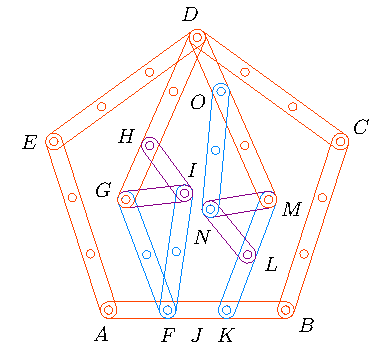
\includegraphics[scale=1.2]{3/penta3-10a}
\caption{Pentagon of size 3 with 10 internal strips. $\overline{DE}:\overline{EA}:\overline{AF} = 3:3:1$. $\overline{DF} = \overline{DK} = \dfrac{\sqrt{46+18\sqrt5}}2$.}
\label{fig:penta3-10a}
\end{figure}

Figure \ref{fig:penta3-10a} show the regular pentagon $A,B,C,D,E$ of size $3$. We know the regular pentagon height is side length times $\dfrac{\sqrt{5+2\sqrt5}}2$ so in this case $\overline{DJ} = \dfrac{3\sqrt{5+2\sqrt5}}2$ and we can calculate $\overline{DF}$:
\begin{align}
\overline{DF} &= \sqrt{(\overline{DJ})^2 + (\overline{FJ})^2}\nonumber\\
 &= \sqrt{\left(\frac{3\sqrt{5+2\sqrt5}}2\right)^2 + \left(\frac{1}2\right)^2}
 = \frac{\sqrt{46+18\sqrt5}}2
\end{align}

\subsubsection{Rigid distance $\dfrac{\sqrt{46+18\sqrt5}}2$}

Our software found several five strips clusters and we use two different which fit inside the pentagon.

We identify two angles $\alpha = \angle{HGI} = \angle{LMN}$ of equilateral triangles and $\beta = \angle{FGI} = \angle{NMO}$ of isoscelles'. Adding the angles we get angles $\angle{DGF} = \angle{DMK} = (\alpha + \beta)$. From equilateral triangle $\triangle{HGI}$ we calculate $\cos\alpha$ and $\sin\alpha$:
\begin{align}
\cos\alpha &= \frac{\frac{\overline{GI}}2}{\overline{GH}} = \frac{\frac{1}2}1 = \frac{1}2\\
\sin\alpha &= \sqrt{1 - \cos^2\alpha} = \sqrt{1 - \left(\frac{1}2\right)^2} = \frac{\sqrt3}2
\end{align}

From isoscelles triangle $\triangle{FGI}$ we calculate $\cos\beta$ and $\sin\beta$:
\begin{align}
\cos\beta &= \frac{\frac{\overline{GI}}2}{\overline{GF}} = \frac{\frac{1}2}{2} = \frac{1}4\\
\sin\beta &= \sqrt{1 - \cos^2\beta} = \sqrt{1 - \left(\frac{1}4\right)^2} = \frac{\sqrt{15}}4
\end{align}

Now we calculate $\cos(\alpha+\beta)$ with the sum identity:
\begin{align}
\cos(\alpha+\beta) &= \cos\alpha\cos\beta - \sin\alpha\sin\beta \nonumber\\
 &= \left(\frac{1}2\right)\left(\frac{1}4\right)
  -\left(\frac{\sqrt3}2\right)\left(\frac{\sqrt{15}}4\right)
 = \frac{1 - 3\sqrt5}8
\end{align}

Finally using the law of cosines we verify distance $\overline{DF}$:
\begin{align}
\overline{DF} &= \sqrt{(\overline{DG})^2 + (\overline{FG}^2)
 - 2(\overline{DG})(\overline{FG})\cos(\alpha+\beta)} \nonumber\\
 &= \sqrt{3^2 + 2^2 - 2(3)(2)\left(\frac{1 - 3\sqrt5}8\right)}
 = \frac{\sqrt{46+18\sqrt5}}2 \quad\blacksquare
\end{align}

\subsection{Size 3 with 14 internal strips $build(3:1)$}

\begin{figure}[H]
\centering
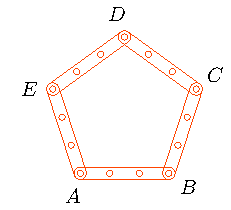
\includegraphics[scale=1.2]{3/penta3-14a}
\caption{Pentagon of size 3 with 14 internal strips. $\overline{AB}:\overline{BD} = 3:1$. $\overline{AD} = \dfrac{\sqrt{34+5\sqrt5}}2$.}
\label{fig:penta3-14a}
\end{figure}

Figure \ref{fig:penta3-14a} show the regular pentagon $A,B',A',C,B$ of size $3$. We know the internal angle of pentagon is $\theta=\dfrac{3\pi}5$ and $\cos\theta=\dfrac{1-\sqrt5}4$ so with the law of cosines we can calculate $\overline{AD}$ and the angle $\angle{BAD}$:
\begin{align}
\overline{AD} &= \sqrt{(\overline{AB})^2 + (\overline{BD})^2
 - 2(\overline{AB})(\overline{BD})\cos\theta} \nonumber\\
 &= \sqrt{3^2 + 1^2 - 2(3)(1)\left(\frac{1-\sqrt5}4\right)} = \frac{\sqrt{34+6\sqrt5}}2\\
\cos(\angle{BAD}) &= \frac{(\overline{AD})^2 + (\overline{AB})^2 - (\overline{BD})^2}
 {2(\overline{AD})(\overline{AB})} \nonumber\\
 &= \frac{\dfrac{34+6\sqrt5}4 + 3^2 - 1^2}{2\left(\dfrac{\sqrt{34+6\sqrt5}}2\right)(3)}
  = \frac{11+\sqrt5}{2\sqrt{34+6\sqrt5}}
\end{align}

\subsubsection{Rigid distance  $\dfrac{\sqrt{34+6\sqrt5}}2$}

Our software found several options to make the distance with five strips but we have to manually add a sixth strip in order to make a cluster narrow enough to fit two times inside the pentagon of size $3$. The result show as the duplicated cluster with vertices $D,E,F,G,H$ of the figure. We are going to prove the cluster's distance $\overline{AD}$ matches the distance alredy calculated.

Noting the pair of adjacent equilateral triangles $\triangle{DGH}$ and $\triangle{EGH}$ we know angle $\angle{DGE} = \dfrac{2\pi}3$ and also $\cos\left(\dfrac{2\pi}3\right) = -\dfrac{1}2$ so we can calculate $\overline{DE}$ and the angle $\alpha \equiv \angle{GDE}$:
\begin{align}
\overline{DE} &= \sqrt{(\overline{DG})^2 + (\overline{GE})^2 
 - 2(\overline{DG})(\overline{GE})\cos(\angle{DGE})}
 = \sqrt{1^2 + 1^2 - 2(1)(1)\left(-\frac{1}2\right)} = \sqrt3\\
\alpha &\equiv = \angle{GED} \nonumber\\
\cos\alpha &= \frac{(\overline{GE})^2 + (\overline{DE})^2 - (\overline{DG})^2}
 {2(\overline{GE})(\overline{DE})}
 = \frac{3 + 1^2 - 1^2}{2(\sqrt3)(1)} = \frac{\sqrt3}2\\
\sin\alpha &= \sqrt{1 - \cos^2\alpha} = \sqrt{1 - \left(\frac{\sqrt3}4\right)^2} 
 = \frac{1}2
\end{align}

From the isoscelles triangle $\triangle{AEF}$ we can calculate angle $\angle{AEF}$ noting $\cos(\angle{AEF}) = \dfrac{\overline{EF}/2}{\overline{AE}} = \dfrac{1/2}{2} = \dfrac{1}4$ so we define angle $\beta \equiv \angle{AEG}$ the supplementary of $\angle{AEF}$ and we get:
\begin{align}
\beta \equiv& \angle{AEG} = \pi - \angle{AEF} \nonumber\\
\cos\beta &= -\cos{\angle{AEF}} = -\frac{1}4 \\
\sin\beta &= \sqrt{1 - \cos^2\beta} = \sqrt{1 - \left(\frac{-1}4\right)^2} = \frac{\sqrt{15}}4
\end{align}

Now we can calculate the angle $\angle{AED} = \alpha + \beta$ with the sum identity and plugin the last sines and cosines:
\begin{align}
\cos(\angle{AED}) &= \cos(\alpha + \beta) \nonumber\\
 &= \cos\alpha\cos\beta - \sin\alpha\sin\beta \nonumber\\
 & = \left(\frac{\sqrt3}2\right)\left(-\frac{1}4\right) 
  - \left(\frac{1}2\right)\left(\frac{\sqrt{15}}4\right) 
  = -\frac{\sqrt3 + \sqrt{15}}8
\end{align}

Finally we calculate $\overline{AD}$ with the law of cosines:
\begin{align}
\overline{AD} &= \sqrt{(\overline{DE})^2 + (\overline{EA})^2 
 - 2(\overline{DE})(\overline{EA})\cos(\angle{AED})} \nonumber\\
 &= \sqrt{3 + 2^2 - 2(\sqrt3)(2)\left(-\frac{\sqrt3 + \sqrt{15}}8\right)} 
 = \frac{\sqrt{34 + 6\sqrt5}}2 \quad\blacksquare
\end{align}

% 4

\section{Pentagons of size 4}

\subsection{Size 4 with 8 internal strips $build(2:4:1:2)$}

\begin{figure}[H]
\centering
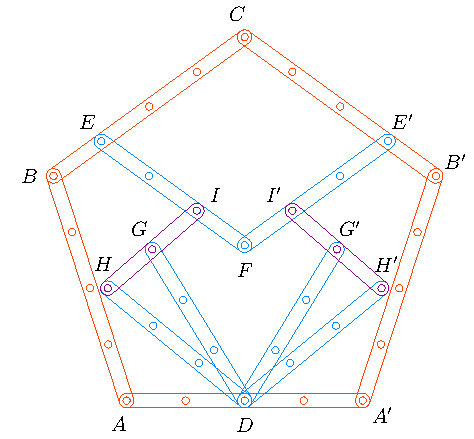
\includegraphics[scale=1.1]{4/penta4-8a}
\caption{Pentagon of size 4 with 6 internal strips. $\overline{DA} : \overline{AB} : \overline{BE} : \overline{EI} = 2:4:1:2$. $\overline{DI} = \sqrt{11}$.}
\label{fig:penta4-8a}
\end{figure}

Figure \ref{fig:penta4-8a} show the regular pentagon $AA'B'CB$ of size $4$. We calculate the distance $\overline{DI}$ assuming vertex $D$ is at origin and calculating abscissa and ordinate of vertex $I$ and knowing $\alpha = \angle{ADB} = \dfrac{3\pi}5$ and $\beta = \angle{B'BE} = \dfrac{\pi}5$. Adding and substracting through vertices $D,A,B,E,I$ we get:
\begin{align}
I_x &= -\overline{DA} - \overline{AB}|\cos\alpha| + \overline{BE}\cos\beta + \overline{EI}\cos\beta \nonumber\\
 &= -2 -(4)\left|-\frac{\sqrt5 - 1}4\right| + (1+2)\left(\frac{\sqrt5+1}4\right)
 = -\frac{1+\sqrt5}4 \\
I_y &= \overline{AB}\sin\alpha + \overline{BE}\sin\beta - \overline{BI}\sin\beta \nonumber\\
 &= (4)\left(\frac{\sqrt{10+2\sqrt5}}4\right) + (1-2)\left(\frac{\sqrt{10-2\sqrt5}}4\right)
 = \frac{4\sqrt{10+2\sqrt5} - \sqrt{10-2\sqrt5}}4 \\
%
\overline{DI} &= \sqrt{(I_x - D_x)^2 + (I_y - I_y)^2} \nonumber\\
 &= \frac{\sqrt{(1+\sqrt5)^2 + (4\sqrt{10+2\sqrt5} - \sqrt{10-2\sqrt5})^2}}4
 = \sqrt{11}
\end{align}

\subsubsection{Rigid distance $\sqrt{11}$}

Our software found several three strips clusters for rigid distance $\sqrt{11}$. We prove the selected cluster $DHGI$ inside the pentagon matches the expected distance. First we calculate the angle $\angle{DHG}$ with the law of cosines and use the value to finally calculate the distance $\overline{DI}$ with again the law of cosines:
\begin{align}
\cos(\angle{DHG}) &= \frac{(\overline{HD})^2 + (\overline{HG})^2 - (\overline{DG})^2}
 {2(\overline{HD})(\overline{HG})} \nonumber\\
 &= \frac{3^2 + 1^2 - 3^2}{2(3)(1)} = \frac{1}6 \\
\overline{DI} &= \sqrt{(\overline{HD})^2 + (\overline{HI})^2
 - 2(\overline{HD})(\overline{HD})\cos(\angle{DHG})} \nonumber\\
 &= \sqrt{3^2 + 2^2 - 2(3)(2)\left(\frac{1}6\right)} = \sqrt{11} \quad\blacksquare
\end{align}

\subsection{Size 4 with 10 internal strips $build(3:4)$}

\begin{figure}[H]
\centering
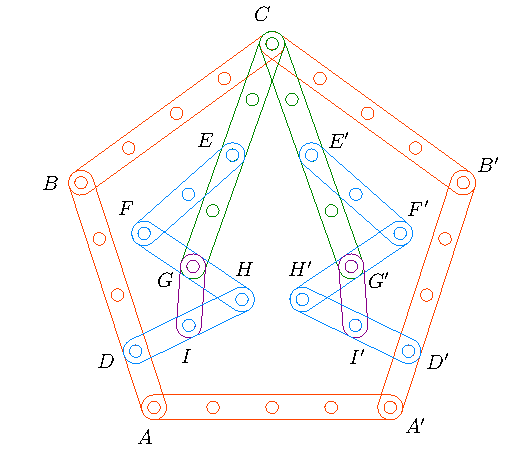
\includegraphics[scale=1.1]{4/penta4-10a}
\caption{Pentagon of size 4 with 10 internal strips. $\overline{CB} : \overline{BD} = 4:3$. $\overline{CD} = \sqrt{19 + 6\sqrt5}$.}
\label{fig:penta4-10a}
\end{figure}

Figure \ref{fig:penta4-10a} show the regular pentagon $A,A',B',C,B$ of size $4$. We know the internal angle of pentagon is $\theta=\angle{CBD}=\dfrac{3\pi}5$ and $\cos\theta=\dfrac{1-\sqrt5}4$ so with the law of cosines we can calculate $\overline{CD}$ and the angle $\angle{DCB}$:
\begin{align}
\overline{CD} &= \sqrt{(\overline{BC})^2 + (\overline{BD})^2
 - 2(\overline{BC})(\overline{BD})\cos\theta} \nonumber\\
 &= \sqrt{4^2 + 3^2 - 2(4)(3)\left(\frac{1-\sqrt5}4\right)} = \sqrt{19+6\sqrt5}\\
%
\cos(\angle{DCB}) &= \frac{(\overline{CD})^2 + (\overline{BC})^2 - (\overline{BD})^2}
 {2(\overline{CD})(\overline{BC})} \nonumber\\
 &= \frac{(19+6\sqrt5) + 4^2 - 3^2}{2\left(\sqrt{19+6\sqrt5}\right)(4)}
  = \frac{13 + 3\sqrt5}{4\sqrt{19+6\sqrt5}}
\end{align}

\subsubsection{Rigid distance  $\sqrt{19+6\sqrt5}$}

Our software found several five strips clusters for rigid distance $\sqrt{19+6\sqrt5}$. We prove selected cluster $CEFGHID$ show in the figure inside the pentagon matches the expected distance. Set the cluster in the coordinate plane such that vertice $G$ is at the origin and vertices $F$ at $(-1,0)$ and vertice $H$ at $(+1,0)$.
Since triangle $\triangle{EFG}$ is isoscelles and $\overline{CG}$ is the double of $\overline{GE}$ we know angle $\angle{CFG} = \frac{\pi}2$ and we can calculate the abscissa and ordinate of vertex $C$:
\begin{align}
C_x &= -\overline{FG} = -1 \\
C_y &= \sqrt{(\overline{CG})^2 - (\overline{FG})^2} = \sqrt{4^2 - 1^2} = \sqrt{15}
\end{align}

Since triangle $\triangle{GHI}$ is equilateral and $\overline{HD}$ is the double of $\overline{HI}$ we know angle $\angle{DGH} = \frac{\pi}2$ and we can calculate the abscissa and ordinate of vertex $D$:
\begin{align}
D_x &= 0 \\
D_y &= -\sqrt{(\overline{HD})^2 - (\overline{GH})^2} = -\sqrt{2^2 - 1^2} = -\sqrt3
\end{align}

Finally we calculate the distance $\overline{CD}$
\begin{align}
\overline{CD} &= \sqrt{(C_x - D_x)^2 + (C_y - D_y)^2} \nonumber\\
 &= \sqrt{(-1 - 0)^2 + (\sqrt{15} + \sqrt{3})^2} = \sqrt{19 + 6\sqrt5} \quad\blacksquare
\end{align}

% 5

\section{Pentagons of size 5}

\subsection{Size 5 with 10 internal strips $build(3,5)$}

\begin{figure}[H]
\centering
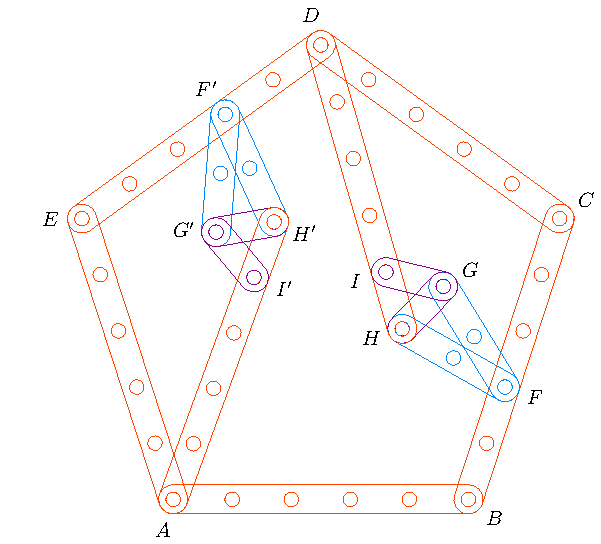
\includegraphics[scale=0.9]{5/penta5-10a}
\caption{Pentagon of size 5 with 10 internal strips. $\overline{FC} : \overline{CD} = 3:5$. $\overline{FD} = \dfrac{\sqrt{106 + 30\sqrt5}}2$.}
\label{fig:penta5-10a}
\end{figure}

\subsubsection{Rigid distance $\dfrac{\sqrt{106 + 30\sqrt5}}2$}

\subsection{Size 5 with 12 internal strips $build(4:5:4)$}

\begin{figure}[H]
\centering
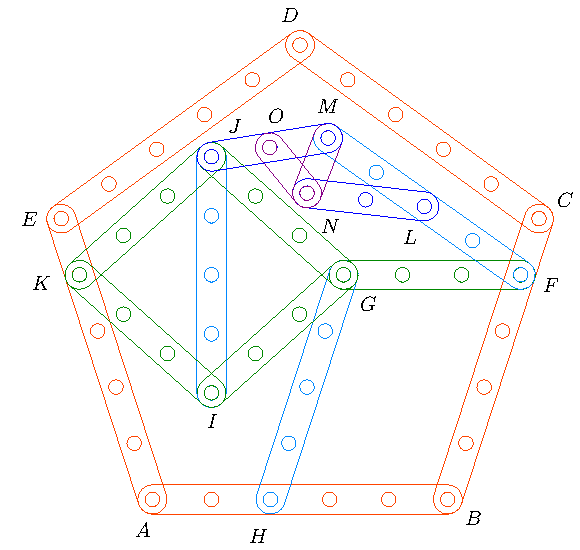
\includegraphics[scale=0.9]{5/penta5-12a}
\caption{Pentagon of size 5 with 12 internal strips. $\overline{FB} : \overline{BA} : \overline{AK} = 4:5:4$ and $\overline{FK} = 3 + 2\sqrt5$. $\overline{FJ} = \sqrt{18+6\sqrt5} = \sqrt3 + \sqrt{15}$.}
\label{fig:penta5-12a}
\end{figure}

\subsubsection{Rigid distances $3+2\sqrt5$ and $\sqrt{18+6\sqrt5} = \sqrt3 + \sqrt{15}$}


% 6

\section{Pentagons of size 6}

\subsection{Size 6 with 6 internal strips $build(4:6:4)$}

\begin{figure}[H]
\centering
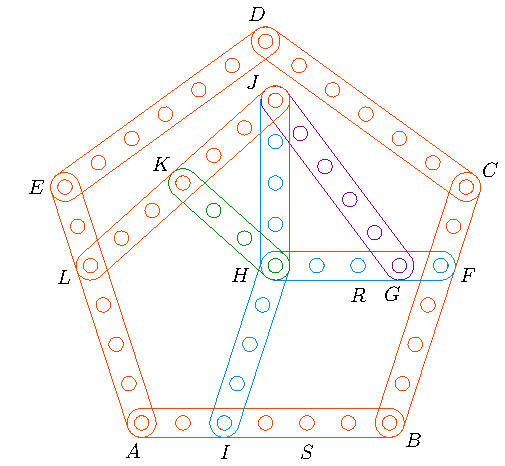
\includegraphics[scale=0.7]{6/penta6-6a}
\caption{Pentagon of size 6 with 6 internal strips. $\overline{FB} : \overline{BA} : \overline{AL} = 4:6:4$. $\overline{FL} = 4 + 2\sqrt5$.}
\label{fig:penta6-6a}
\end{figure}

\subsubsection{Rigid distance $4 + 2\sqrt5$}

\subsection{Size 6 with 8 internal strips $build(6:6:3:4)$}

\begin{figure}[H]
\centering
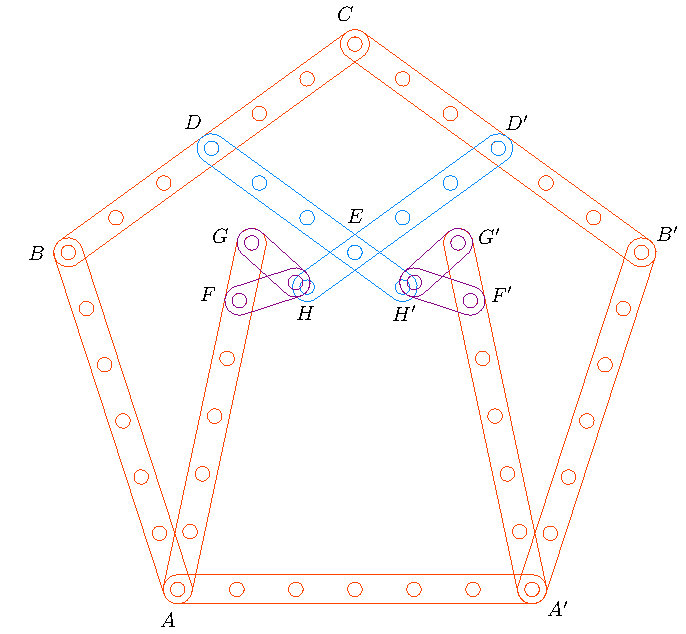
\includegraphics[scale=0.7]{6/penta6-8a}
\caption{Pentagon of size 6 with 8 internal strips. $\overline{A'A} : \overline{AB} : \overline{BD} : \overline{DF'} = 6:6:3:4$ and $\overline{A'F'} = \sqrt{31}$.}
\label{fig:penta6-6a}
\end{figure}

\subsubsection{Rigid distance $\sqrt{31}$}

\subsection{Size 6 with 10 internal strips $build(5:6)$}

\begin{figure}[H]
\centering
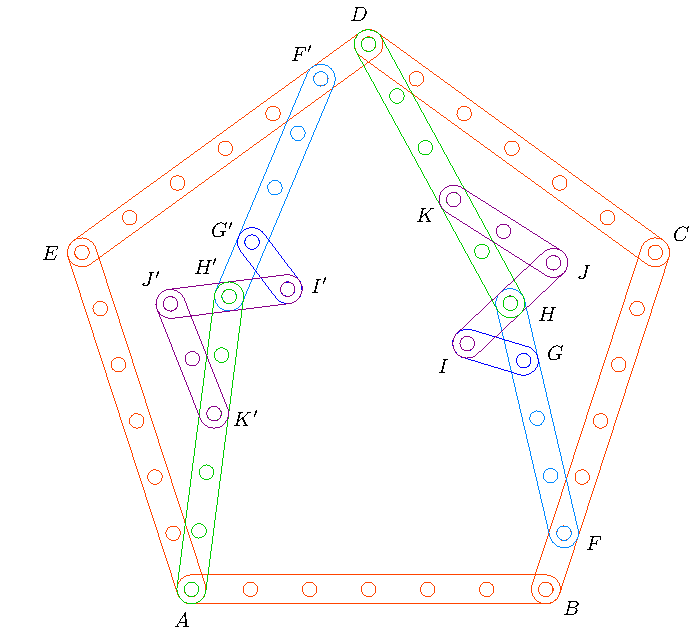
\includegraphics[scale=0.7]{6/penta6-10a}
\caption{Pentagon of size 6 with 10 internal strips. $\overline{FC} : \overline{CD} = 5:6$. $\overline{FD} = \sqrt{46 + 15\sqrt5}$.}
\label{fig:penta6-10a}
\end{figure}

\subsubsection{Rigid distance $\sqrt{46 + 15\sqrt5}$}

\subsection{Size 6 with 12 internal strips $build(0:6:4:2)$}

\begin{figure}[H]
\centering
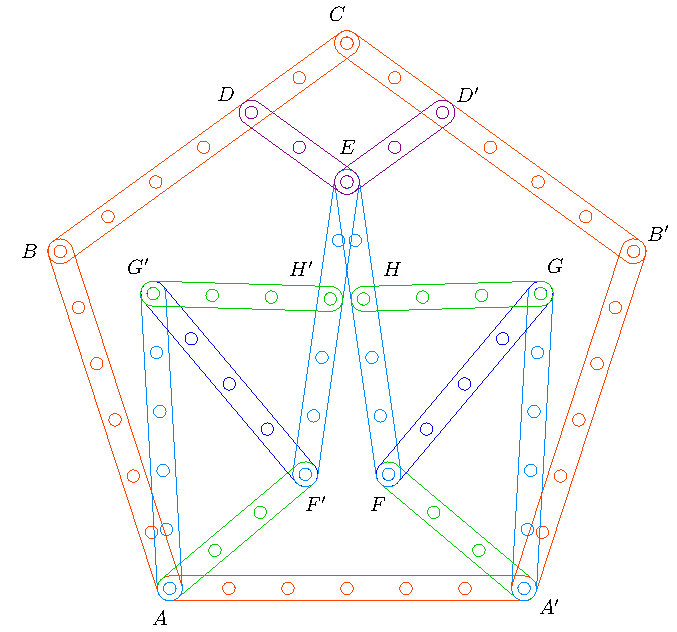
\includegraphics[scale=0.7]{6/penta6-12a}
\caption{Pentagon of size 6 with 12 internal strips. $\overline{AA}:\overline{AB}:\overline{BD}:\overline{DE} = 0:6:4:2$ and $AE = \sqrt{34 + 10\sqrt5}$} 
\label{fig:penta6-12a}
\end{figure}

\subsubsection{Rigid distance $\sqrt{34 + 10\sqrt5}$}



% 7

\section{Pentagons of size 7}

\subsection{Size 7 with 6 internal strips $build(6:7:6)$}

\begin{figure}[H]
\centering
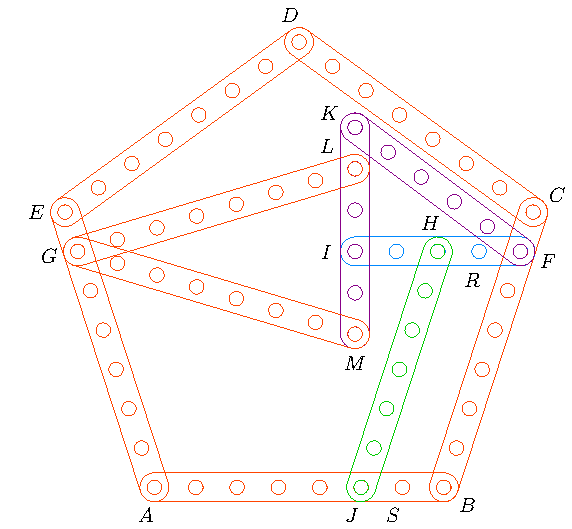
\includegraphics[scale=0.7]{7/penta7-6a}
\caption{Pentagon of size 7 with 6 internal strips. $\overline{FC} : \overline{CD} : \overline{} = 6:7:6$. $\overline{FD} = 4 + 3\sqrt5$.}
\label{fig:penta7-6a}
\end{figure}

\subsubsection{Rigid distance $4 + 3\sqrt5$}


\subsection{Size 7 with 10 internal strips $build(6,7)$}

\begin{figure}[H]
\centering
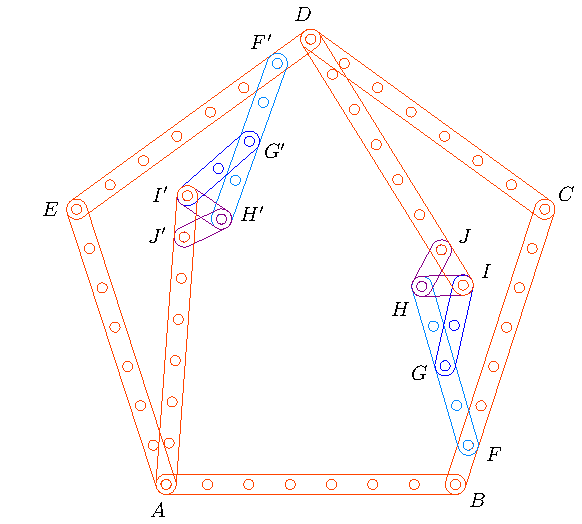
\includegraphics[scale=0.7]{7/penta7-10a}
\caption{Pentagon of size 7 with 10 internal strips. $\overline{FC}:\overline{CD} = 6:7$. $\overline{FD} = \sqrt{64 + 21\sqrt5}$.}
\label{fig:penta7-10a}
\end{figure}

\subsubsection{Rigid distance $\sqrt{64 + 21\sqrt5}$}

\subsection{Size 7 with 14 internal strips}

\begin{figure}[H]
\centering
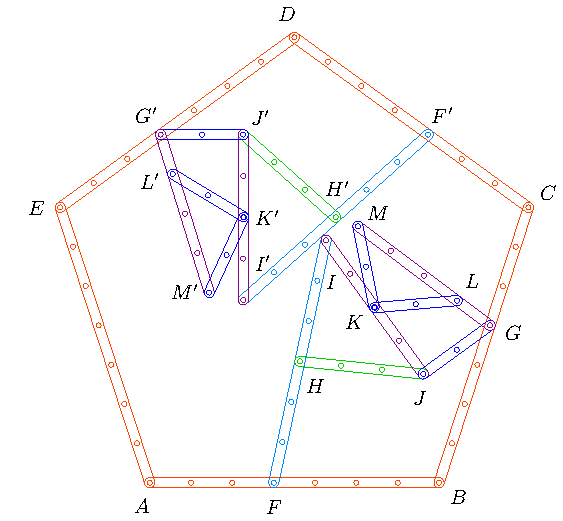
\includegraphics[scale=0.8]{7/penta7-14a}
\caption{Pentagon of size 7 with 14 internal strips. $\overline{FB} : \overline{BG} = 4:4$ and $\overline{FG} = 2 + 2\sqrt5$.}
\label{fig:penta7-14a}
\end{figure}
%
\subsubsection{Rigid distance $2 + 2\sqrt5$}


% 8

\section{Pentagons of size 8}

\subsection{Size 8 with 6 internal strips $build(8:8)$}

\begin{figure}[H]
\centering
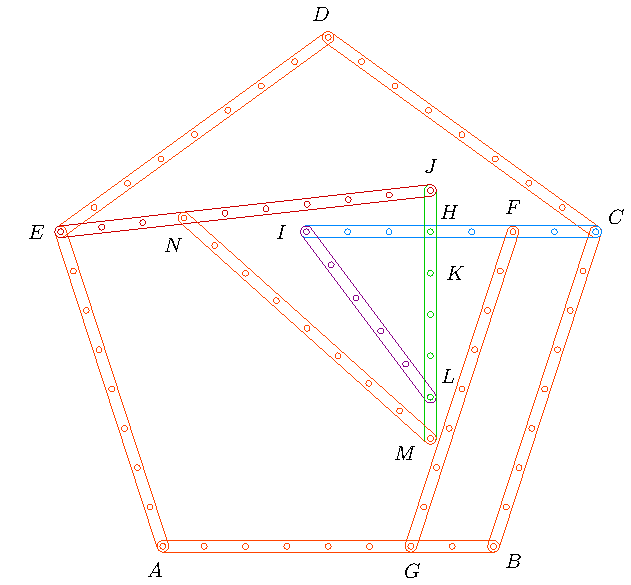
\includegraphics[scale=0.8]{8/penta8-6a}
\caption{Pentagon of size 8 with 6 internal strips. $\overline{CD} : \overline{DE} = 8:8$. $\overline{FD} = 4 + 4\sqrt5$.}
\label{fig:penta8-6a}
\end{figure}

Figure \ref{fig:penta8-6a} show regular pentagon $ABCDE$ of size 8. We know the pentagon width like $\overline{CE}$ is $\frac{1+\sqrt5}2$ times the side of the pentagon so here we have $\overline{CE} = 4+4\sqrt5$.

\subsubsection{Rigid distance $4 + 4\sqrt5$}

From the figure consider triangle $\triangle{NJM}$ and calculate with the law of cosines angle $\theta = \angle{NJM}$:
\begin{align}
\cos\theta = \frac{(\overline{JM})^2 + (\overline{JN})^2 
 - (\overline{MN})^2}{2(\overline{JM})(\overline{JN})}
 &= \frac{6^2 + 6^2 - 8^2}{2(6)(6)} = \frac{1}9
\end{align}
Since $\dfrac{\overline{EH}}{\overline{EJ}} = \sin\theta$ we have:
\begin{align}
\overline{EH} &= (\overline{EJ})\sin\theta
 = 9\sqrt{1-\cos^2\theta} 
 = 9\sqrt{1-\left(\frac{1}9\right)^2} = 4\sqrt5
\end{align}

Since $(\overline{EJ})^2 = (\overline{EH})^2 + (\overline{HJ})^2 \mapsto 9^2 = 16(5) + 1$ we conclude we have the right angle $\angle{EHJ} = \frac{\pi}2$. By inspection we have a second right angle $\angle{IHL} = \frac{\pi}2$ formed by the Pythagorean triangle $\triangle{HIL}$ and a third one $\angle{LHC} = \frac{\pi}2$ since is supplementary of $\angle{IHL}$. With the right angles we conclude vertices $E,H,C$ are colinear so the distance $\overline{EH} = \overline{EH} + \overline{HC} = 4\sqrt{5} + 4$ $\blacksquare$.
The strip $\overline{FG}$ keeps rigid the vertices $A$ and $B$.

\subsection{Size 8 with 8 internal strips $build(4:8:2:4)$ and $build(4:8:4:6)$}

\begin{figure}[H]
\centering
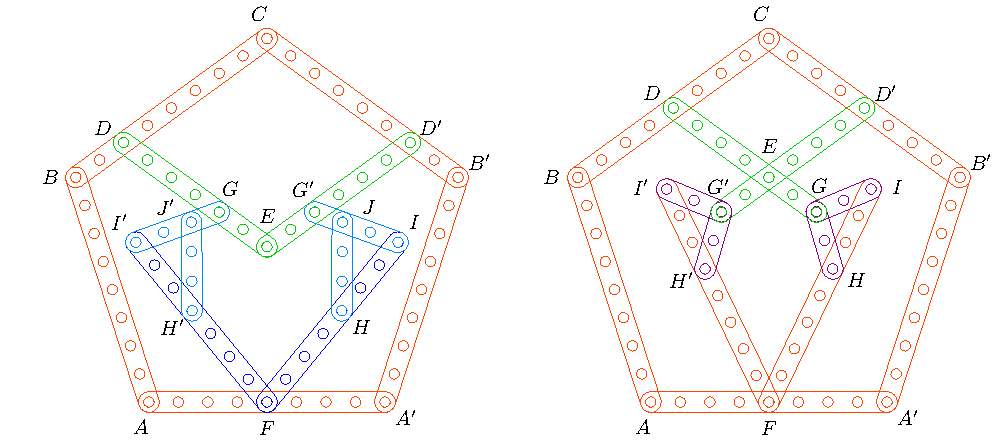
\includegraphics[scale=1]{8/penta8-8a}
\caption{Pentagons of size 8 with 8 internal strips. For the pentagon variation 1 at the left $\overline{FA}:\overline{AB}:\overline{BD}:\overline{DG} = 4:8:2:4$ and $\overline{FG}=2\sqrt{11}$. For the pentagon variation 2 at the right $\overline{AF}:\overline{AB}:\overline{BD}:\overline{DG} = 4:8:4:6$ and $\overline{FG}=2\sqrt{11}$.}
\label{fig:penta8-8a}
\end{figure}

Figure \ref{fig:penta8-8a} show two rigid regular pentagons $A,A',B',C,B$ of size $9$. For the variation 1 at the left and assuming vertice $F$ is at the origin we calculate the distance $\overline{FG}$ using the abscissas and ordinates following the vertices $F,A,B,D,G$ for a regular pentagon angles $3\pi/5$, $\beta=\pi/5$:
\begin{align}
FI_x &= -\overline{AF} - \overline{AB}\cos\alpha + (\overline{BD} + \overline{DI})\cos\beta\nonumber\\
 &= -4 + (8)\frac{1-\sqrt5}4 + (2+4)\frac{\sqrt5+1}4 = -\frac{2+2\sqrt5}4\\
FI_y &= \overline{AB}\sin\alpha + (\overline{BD}-\overline{DI})\sin\beta\nonumber\\
 &= (8)\frac{\sqrt{10+2\sqrt5}}4 + (2-4)\frac{\sqrt{10-2\sqrt5}}4
 = \frac{8\sqrt{10+2\sqrt5} - 2\sqrt{10-2\sqrt5}}4\\
\overline{FI} &= \sqrt{(FI_x)^2 + (FI_y)^2}\nonumber\\
 &= \frac{\sqrt{(2+2\sqrt5)^2 + (8\sqrt{10+2\sqrt5} - 2\sqrt{10-2\sqrt5})^2}}4
 = \frac{\sqrt{704}}4 = 2\sqrt{11}
\end{align}
For the variation 2 at the right vertices $G,G'$ switch positions of those of variation 1 and in both variations we have $\overline{FG} = \overline{FG'} = 2\sqrt{11}$.


\subsubsection{Rigid distances $2\sqrt{11}$}

Our software found several options. For the variation 1 at the left of the figure consider the cluster $FHIJG'$. Within the isoscelles triangle $\triangle{HIJ}$ we calculate the cosine of angle $\theta = \angle{JIH}$ and use it with the law of cosines to calculate $\overline{FG'}$:
\begin{align}
\cos\theta &= \frac{\overline{IJ}/2}{\overline{IH}} = \frac{1}3 \nonumber\\
\overline{FG'} &= \sqrt{(\overline{FI})^2 + (\overline{IG'})^2 
 - 2(\overline{FI})(\overline{IG'})\cos\theta} \nonumber\\
 &= \sqrt{7^2 + 3^2 - 2(7)(3)\frac{1}3} = 2\sqrt{11} \quad\blacksquare
\end{align}

For the variation 2 at the right of the figure consider the cluster $FHIG$. Within the isoscelles triangle $GIH$ we calculate the cosine of angle $\phi = \angle{HIG}$ and use it with the law of cosines to calculate $\overline{FG}$:
\begin{align}
\cos\phi &= \frac{\overline{HI}/2}{\overline{GI}} = \frac{3}4 \nonumber\\
\overline{FH} &= \sqrt{(\overline{FI})^2 + (\overline{GI})^2
 - 2(\overline{FI})(\overline{GI})\cos\phi} \nonumber\\
 &= \sqrt{8^2 + 2^2 - 2(8)(2)\frac{3}4} = 2\sqrt{11} \quad\blacksquare
\end{align}

\subsection{Size 8 with 10 internal strips $build(4:8)$}

\begin{figure}[H]
\centering
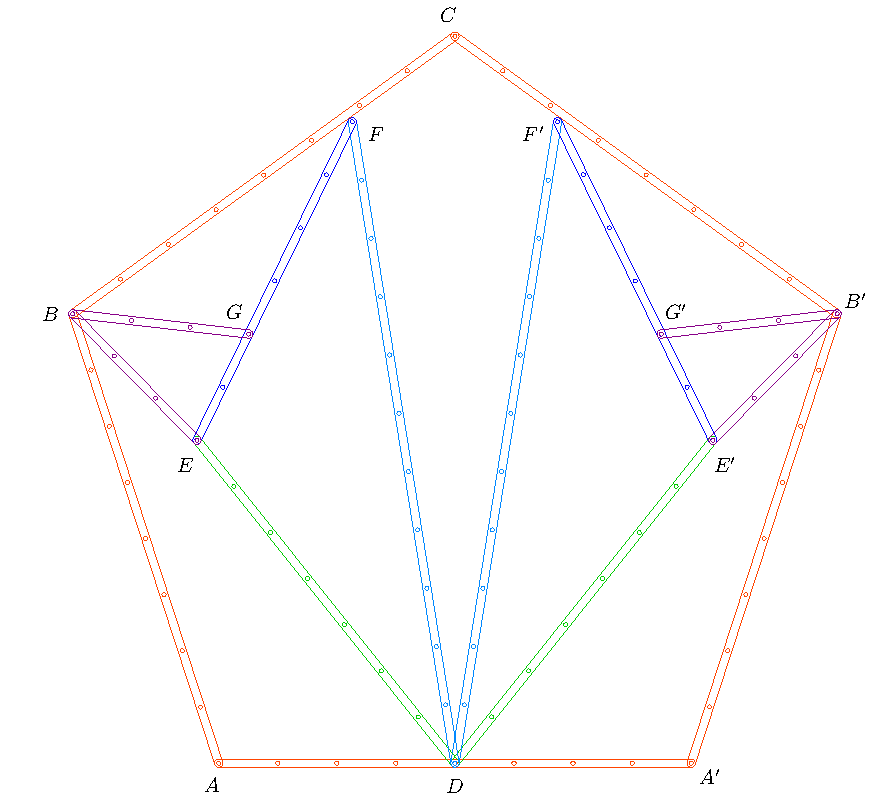
\includegraphics[scale=1]{8/penta8-10a}
\caption{Pentagon of size 8 with 10 internal strips. $\overline{DA}:\overline{AB} = 4:8$ and $\overline{DB} = 4\sqrt{4 + \sqrt5}$}
\label{fig:penta8-10a}
\end{figure}

Figure \ref{fig:penta8-10a} show pentagon $AA'B'CB$ of size $8$. We use the law of cosines to calculate distance $\overline{DB}$ knowing $\theta = \angle{DAB} = \frac{3\pi}5$ and $\cos\theta = \frac{1-\sqrt5}4$:
\begin{align}
\overline{DB} &= \sqrt{(\overline{AD})^2 + (\overline{AB})^2
 - 2(\overline{AD})(\overline{AB})\cos\theta} \nonumber\\
 &= \sqrt{4^2 + 8^2 - 2(4)(8)\frac{1-\sqrt5}4} = 4\sqrt{4 + \sqrt5}
\end{align}

\subsubsection{Rigid distance $4\sqrt{4 + \sqrt5}$}

Our software found few solutions but the cluster $DEBGF$ shown in the figure fit (hardly) inside the pentagon. We calculate angles around vertice $E$ $\alpha = \angle{DEF}$ with the law of cosines and $\beta = \angle{BEG}$ whitin the isoscelles triangle $\triangle{BEG}$:
\begin{align}
\cos\alpha &= \frac{(\overline{DE})^2 + (\overline{EF})^2 - (\overline{DF})^2}
 {2(\overline{DE})(\overline{EF})} 
 = \frac{7^2 + 6^2 - 11^2}{2(7)(6)} = -\frac{3}7 \\
\sin\alpha &= \sqrt{1 - \cos^2\alpha}
 = \sqrt{1 - \left(-\frac{3}{7}\right)^2} = \frac{2\sqrt{10}}7 \\
\cos\beta &= \frac{\frac{\overline{EG}}2}{\overline{EB}}
 = \frac{\frac{2}{2}}{3} = \frac{1}3\\
\sin\beta &= \sqrt{1 - \sin^2{\beta}}
 = \sqrt{1 - \left(\frac{1}3\right)^2} = \frac{2\sqrt2}3
\end{align}

Now we calculate the angle $\angle{DEB} = \gamma = \alpha + \beta$ using the cosines sum identity:
\begin{align}
\cos\gamma &= \cos(\alpha + \beta)
 = \cos\alpha\cos\beta - \sin\alpha\sin\beta \nonumber\\
 &= \left(-\frac{3}7\right)\left(\frac{1}3\right)
  - \left(\frac{2\sqrt{10}}7\right)\left(\frac{2\sqrt2}3\right)
  = -\frac{3 + 8\sqrt{5}}{21}
\end{align}

Finally we calculate the distance $\overline{DB}$ using previous angle $\gamma$:
\begin{align}
\overline{DB} &= \sqrt{(\overline{DE})^2 + (\overline{EB})^2
 - 2(\overline{DE})(\overline{EB})\cos\gamma} \nonumber\\
 &= \sqrt{7^2 + 3^2 - 2(7)(3)\left(-\frac{3 + 8\sqrt{5}}{21}\right)} 
 = 4\sqrt{4 + \sqrt5} \quad\blacksquare
\end{align}

\subsection{Size 8 with 10 internal strips $build(7:8)$}

\begin{figure}[H]
\centering
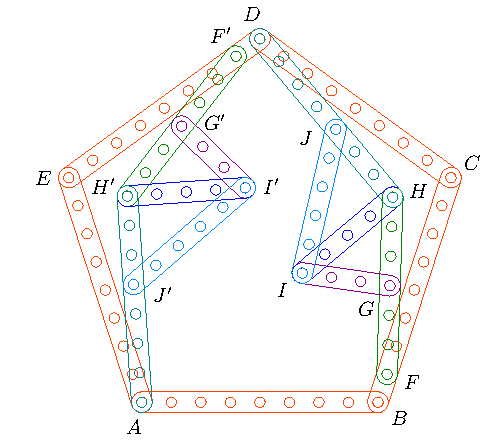
\includegraphics[scale=1.1]{8/penta8-10b}
\caption{Pentagon of size 8 with 10 internal strips. $\overline{FC}:\overline{CD} = 7:8$ and $\overline{CD} = \sqrt{85 + 28\sqrt5}$}
\label{fig:penta8-10b}
\end{figure}

Figure \ref{fig:penta8-10b} show pentagon $ABCDE$ of size $8$. We use the law of cosines to calculate distance $\overline{FD}$ knowing $\theta = \angle{FCD} = \frac{3\pi}5$ and $\cos\theta = \frac{1-\sqrt5}4$:
\begin{align}
\overline{FC} &= \sqrt{(\overline{FC})^2 + (\overline{CD})^2
 - 2(\overline{FC})(\overline{CD})\cos\theta} \nonumber\\
 &= \sqrt{7^2 + 8^2 - 2(7)(8)\frac{1-\sqrt5}4} = \sqrt{85 + 28\sqrt5}
\end{align}

\subsubsection{Rigid distance $\sqrt{85 + 28\sqrt5}$}

Our software found several solutions, consider the cluster $FGHIJD$ in the figure. Assume vertice $I$ is at the origin and vertice $H$ is at coordinate $(4,0)$. Since triangle $\triangle{HIG}$ is isoscelles and $\overline{HF}$ is the double of $\overline{IG}$ then $\overline{IF} = \sqrt{(\overline{HF})^2 - (\overline{IH})^2} = \sqrt{6^2 - 4^2} = 2\sqrt{5}$ and the coordinates of vertice $F(x,y)$ are $(0,\overline{IF}) = (0,-2\sqrt5)$. Since the Pythagorean triangle $\triangle{HIJ}$ we have a right angle $\angle{IHD} = \frac{\pi}2$ and then the coordinates of vertice $D(x,y)$ are $(\overline{IH},\overline{HD}) = (4,7)$. Finally we calculat the distance $\overline{FD}$:
\begin{align}
\overline{FD} &= \sqrt{(F_x - D_x)^2 + (F_y - D_y)^2 } \nonumber\\
 &= \sqrt{(0 - 4)^2 + (-2\sqrt5 - 7)^2} = \sqrt{85 + 28\sqrt5} \quad \blacksquare
\end{align}

\subsection{Size 8 with 10 internal strips $build(8:8)$ and $build(4:8:4)$}

\begin{figure}[H]
\centering
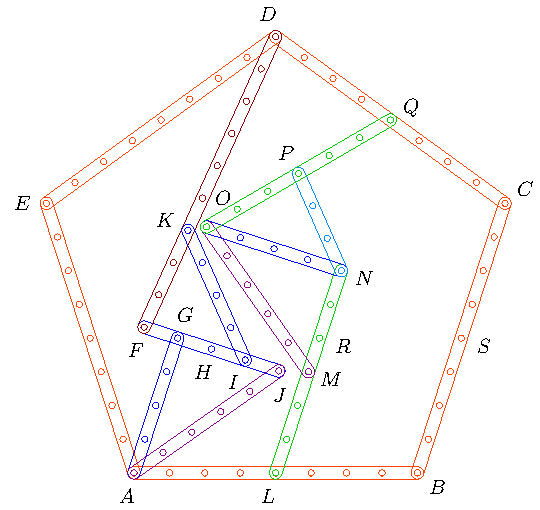
\includegraphics[scale=1]{8/penta8-10c}
\caption{Pentagon of size 8 with 10 internal strips. $\overline{AE}:\overline{ED} = 8:8$ and $\overline{AD} = 4 + 4\sqrt5$. $\overline{LB}:\overline{BC}:\overline{CQ} = 4:8:4$ and $\overline{LQ} = 6 + 2\sqrt5$.}
\label{fig:penta8-10c}
\end{figure}

Figure \ref{fig:penta8-10c} show pentagon $ABCDE$ of size $8$. We have a width $\overline{AD}$ that we know equals the side times $\frac{1+\sqrt5}2$ so we have here:
\begin{align}
\overline{AD} = 8\left(\dfrac{1+\sqrt5}2\right) = 4 + 4\sqrt5
\end{align}
We have a smaller pentagon of side $4$ with a semi-perimeter $\overline{RS},\overline{SC},\overline{CQ}$ with width $\overline{RS} = 4\left(\frac{1+\sqrt5}2\right) = 2 + 2\sqrt5$ so we have:
\begin{align}
\overline{LQ} = \overline{LR} + \overline{RQ} = 4 + 2 + 2\sqrt5 = 6 + 2\sqrt5
\end{align}

\subsubsection{Rigid distances $4 + 4\sqrt5$ and $6 + 2\sqrt5$}

From the last figure we have a (partial) isoscelles triangle $\triangle{FHD}$ where $\alpha = \angle{DFG} = \dfrac{\overline{FG}}{\overline{FD}} = \dfrac{1}9$. The (missing) strip $\overline{HD}$ is substituted by strip $\overline{IK}$ since triangle $\triangle{FIK}$ internal angle $\angle{IFK}$ matches $\alpha$ after using the law of cosines:
\begin{align}
\cos(\angle{IFK}) &= \frac{(\overline{FK})^2 + (\overline{FI})^2 - (\overline{IK})^2}
 {2(\overline{FK})(\overline{FI})} 
 = \frac{3^2 + 3^2 - 4^2}{2(3)(3)}
= \frac{1}9 \quad \blacksquare
\end{align}

Angle $\angle{HGD}=\frac{\pi}2$ since $\triangle{FHD}$ is isoscelles and also $\angle{AGJ} = \frac{\pi}2$ since triangle $\triangle{AGJ}$ is Pythagorean so vertices $A,G,D$ are collinear and then we can get $\overline{AD}$:
\begin{align}
\overline{AD} &= \overline{AG} + \overline{GD} \nonumber\\
 &= 4 + \sqrt{(\overline{FD})^2 - (\overline{FG})^2}
 = 4 + \sqrt{9^2 - 1^2} = 4 + 4\sqrt5 \quad \blacksquare
\end{align}

From the last figure we see triangle $\triangle{NOP}$ is isoscelles and that strip $\overline{OQ}$ is the double of strip $\overline{PN}$ so angle $\angle{ONQ} = \frac{\pi}2$ and we can calculate $\overline{NQ} = \sqrt{(\overline{OQ})^2 - (\overline{ON})^2} = \sqrt{6^2 - 4^2} = 2\sqrt5$. Also angle $\angle{MNO} = \frac{\pi}2$ since triangle $\triangle{MNO}$ is Pythagorean so vertices $M,N,Q$ are collinear and we can get $\overline{LQ}$:
\begin{align}
\overline{LQ} &= \overline{LN} + \overline{NQ} \nonumber\\
 &= 6 + 2\sqrt5 \quad \blacksquare
\end{align}


% 9

\section{Pentagons of size 9}

\subsection{Size 9 with 6 internal strips $build(8:9:8)$}

\begin{figure}[H]
 \centering
 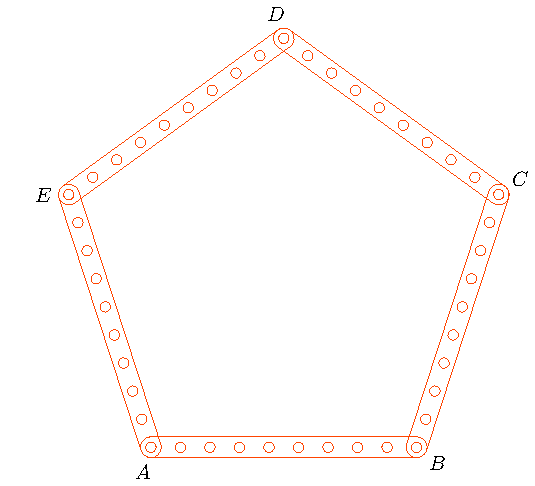
\includegraphics[scale=0.95]{9/penta9a}
 \caption{Pentagon size 9 with six internal strips. $\overline{FB}:\overline{BA}:\overline{AG} = 8:9:8$. $\overline{FG}=5+4\sqrt5$. }
 \label{fig:penta9a}
\end{figure}

Figure \ref{fig:penta9a} show a rigid regular pentagon $A,B,C,D,E$ of size $9$. The regular pentagon distance $\overline{CE}$ is called width and equals $\dfrac{1+\sqrt5}{2}\overline{AB}$. Is easy to note the distance $\overline{FG}$ equals the width of smaller pentagon size $9-1=8$ plus $1$. So we have:
\begin{align}
\overline{FG} &= \frac{1+\sqrt5}{2}(\overline{BC}-\overline{FC}) + \overline{FC}\nonumber\\
 &= \frac{1+\sqrt5}{2}(9-1) + 1 = 5 + 4\sqrt5
\end{align}

\subsubsection{Rigid distance $5 + 4\sqrt5$}

From the figure we see two right angles. Angle $\angle{GJK}=\frac{\pi}2$ because we have a Pythagorean triangle $\triangle{HJK}$. Angle $\angle{FJM}=\frac{\pi}2$ because we have an isosceles triangle $\triangle{FLM}$. The two right angles share vertice $J$ so vertices $G,J,F$ are collinear. First we calculate the distance $\overline{JF} = \sqrt{(LF)^2 - (LJ)^2} = \sqrt{9^2-1^2} = 4\sqrt5$ and finally the distance $\overline{GF} = \overline{GJ} + \overline{JF} = 5 + 4\sqrt5$ which matches the value in last equation above $\blacksquare$. To make rigid the pentagon we add strip $\overline{IN}$ parallel to side $\overline{GA}$.

\subsection{Size 9 with 8 internal strips $build(3,9,3,5)$}

\begin{figure}[H]
 \centering
 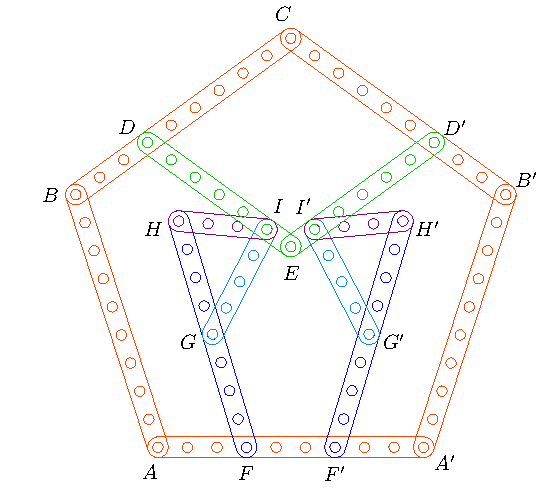
\includegraphics[scale=0.95]{9/penta9-8a}
 \caption{Pentagon size 9 with 8 strips variation 1. $\overline{FA}:\overline{AB}:\overline{BD}:\overline{DI} = 3:9:3:5$. $\overline{FI} = \sqrt{55}$.}
 \label{fig:penta9-8a}
\end{figure}

Figure \ref{fig:penta9-8a} show a rigid regular pentagon $A,A',B',C,B$ of size $9$. First we calculate the distance $\overline{FI}$ using the abscissas and ordinates following the vertices $F,A,B,D,I$ for a regular pentagon angles $\alpha=\dfrac{3\pi}5, \beta=\dfrac{\pi}5$:
\begin{align}
FI_x &= -\overline{AF} - \overline{AB}\cos\alpha + (\overline{BD} + \overline{DI})\cos\beta\nonumber\\
 &= -3 + (9)\frac{1-\sqrt5}4 + (3+5)\frac{\sqrt5+1}4 = \frac{5-\sqrt5}4\\
FI_y &= \overline{AB}\sin\alpha + (\overline{BD}-\overline{DI})\sin\beta\nonumber\\
 &= (9)\frac{\sqrt{10+2\sqrt5}}4 + (3-5)\frac{\sqrt{10-2\sqrt5}}4
 = \frac{9\sqrt{10+2\sqrt5} - 2\sqrt{10-2\sqrt5}}4\\
\overline{FI} &= \sqrt{(FI_x)^2 + (FI_y)^2}\nonumber\\
 &= \frac{\sqrt{(5-\sqrt5)^2 + (9\sqrt{10+2\sqrt5} - 2\sqrt{10-2\sqrt5})^2}}4
 = \frac{\sqrt{880}}4 = \sqrt{55}
\end{align}

\subsubsection{Rigid distance $\sqrt{55}$}

By software we find several options for the distance and we use the one shown in the figure.
We calculate the distance $\overline{FI}$ made rigid by cluster $F,G,H,I$. We have an isoscelles triangle $\triangle{GHI}$ and $\overline{FH}=2\overline{GH}$ so we have a right triangle $\angle{FIH}=\frac{\pi}2$ so: \begin{align}
\overline{FI} &= \sqrt{(\overline{FH})^2 - (\overline{HI})^2}\nonumber\\
 &= \sqrt{8^2 - 3^2} = \sqrt{55} \quad\blacksquare
\end{align}

\subsection{Size 9 with 8 internal strips $build(3,9,1,4)$ and $build(6,9,6,8)$}

\begin{figure}[H]
 \centering
 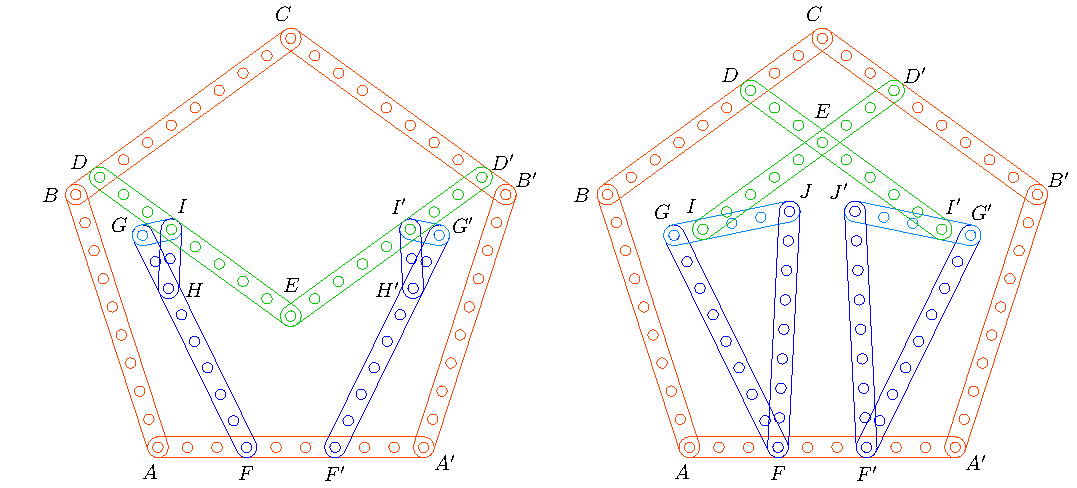
\includegraphics[scale=0.95]{9/penta9-8b}
 \caption{Regular pentagons size 9 made rigid with 8 strips variations 2 and 3. At the left we have $\overline{FA}:\overline{AB}:\overline{BD}:\overline{DI} = 3:9:1:4$ and $\overline{FI} = \sqrt{61}$. At the right we have $\overline{F'A}:\overline{AB}:\overline{BD}:\overline{DI'} = 6:9:6:8$ and $\overline{F'I'}=\sqrt{61}$.}
 \label{fig:penta9-8b}
\end{figure}

Figure \ref{fig:penta9-8b} show two rigid pentagons $A,A',B',C,B'$ of size $9$. The pentagon at the left is called variation 2 and the right one variation 3. Both variations have the vertices $I,I'$ at the same positions and the same distance $\overline{FI}$ which first we calculate using the abscissas and ordinates following the vertices $F,A,B,D,I$ of the variation 2 for a regular pentagon angles $\alpha=\dfrac{3\pi}5, \beta=\dfrac{\pi}5$:
\begin{align}
FI_x &= -\overline{AF} - \overline{AB}\cos\alpha + (\overline{BD} + \overline{DI})\cos\beta\nonumber\\
 &= -3 + (9)\frac{1-\sqrt5}4 + (1+3)\frac{\sqrt5+1}4 = \frac{1-5\sqrt5}4\\
FI_y &= \overline{AB}\sin\alpha + (\overline{BD}-\overline{DI})\sin\beta\nonumber\\
 &= (9)\frac{\sqrt{10+2\sqrt5}}4 + (1-3)\frac{\sqrt{10-2\sqrt5}}4
 = \frac{9\sqrt{10+2\sqrt5} - 2\sqrt{10-2\sqrt5}}4\\
\overline{FI} &= \sqrt{(FI_x)^2 + (FI_y)^2}\nonumber\\
 &= \frac{\sqrt{(1-\sqrt5)^2 + (9\sqrt{10+2\sqrt5} - 2\sqrt{10-2\sqrt5})^2}}4
 = \frac{\sqrt{976}}4 = \sqrt{61}
\end{align}

\subsubsection{Rigid distance $\sqrt{61}$}

Our software found several clusters and we use two different for each variation. We  calculate the distance $\overline{FI}$ made rigid by clusters $F,G,H,I$ or $F,G,I,J$ since in both variations we have the same $\overline{GF}$ and same angles $\angle{FGI}=\angle{FJG}$. With the law of cosines first we calculate $\cos(\angle{FJG})$ and then $\overline{FI}$:
\begin{align}
\cos(\angle{FJG}) &= \frac{\overline{FJ}^2 + \overline{JG}^2 - \overline{GF}^2}
 {2(\overline{FJ})(\overline{JG})}
 = \frac{8^2 + 4^2 - 8^2}{2(8)(4)} = \frac{1}4\nonumber\\
\overline{FI} &= \sqrt{\overline{IJ}^2 + \overline{FJ}^2 
 - 2(\overline{IJ})(\overline{FJ})\cos(\angle{FJG})}
 = \sqrt{3^2 + 8^2 - 2(3)(8)\left(\dfrac{1}4\right)} = \sqrt{61} \quad\blacksquare
\end{align}

\subsection{Size 9 with 10 internal strips $build(4:9)$ and $build(5:9)$}

\begin{figure}[H]
 \centering
 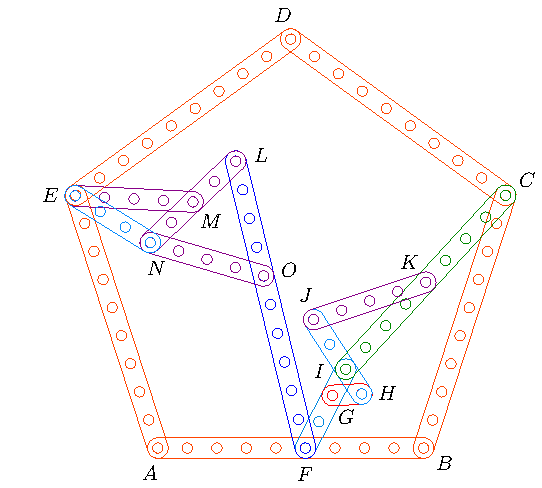
\includegraphics[scale=0.9]{9/penta9b}
 \caption{Pentagons size 9 with two 10 internal strips. For the cluster of the left we have $\overline{FA}:\overline{AE} = 5:9$ and $\overline{FE} = \dfrac{\sqrt{334 + 90\sqrt5}}2$. For the cluster at the right we have $\overline{FB}:\overline{BC} = 4:9$ and $\overline{FC}=\sqrt{79 + 18\sqrt5}$.}
 \label{fig:penta9b}
\end{figure}

Figure \ref{fig:penta9b} show a regular pentagon $A,B,C,D,E$ of size $9$ made it rigid with the help of clusters fixing the distances $\overline{CF}$ and $\overline{EF}$. Pentagon size $9$ is the smaller one with diagonals where consecutive side segments fractions are $\overline{BF} / \overline{BC} =\dfrac{4}9$ and $\overline{AF} / \overline{AE} = \dfrac{5}9$. We calculate the diagonals $\overline{CF}$, $\overline{EF}$ and the angles to side $\overline{AB}$ using the law of cosines and the internal pentagon angle $\theta=\angle{FBC}=\angle{FAE}=\frac{3\pi}5$ where $\cos\theta = \frac{1-\sqrt5}4$. Diagonal $\overline{CF}$:
\begin{align}
\overline{CF} &= \sqrt{
 \overline{BC}^2 + \overline{BF}^2 - 2(\overline{BC})(\overline{BF})\cos\theta } \nonumber\\
 &= \sqrt{9^2 + 4^2 - 2(9)(4)\left(\frac{1-\sqrt5}4\right)} = \sqrt{79 + 18\sqrt5}\\
%
\cos(\angle{CFB}) &= 
 \frac{\overline{CF}^2 + \overline{BF}^2 - \overline{BC}^2}{2(\overline{CF})(\overline{BF})}
 = \frac{79 + 18\sqrt5 + 4^2 - 9^2}{2(\sqrt{79 + 18\sqrt5})(4)}
 = \frac{7 + 9\sqrt5}{4\sqrt{79 + 18\sqrt5}}
\end{align}

Diagonal $\overline{EF}$:
\begin{align}
\overline{EF} &= \sqrt{
 \overline{AE}^2 + \overline{AF}^2 - 2(\overline{AE})(\overline{AF})\cos\theta} \nonumber\\
 &= \sqrt{9^2 + 5^2 - 2(9)(5)\left(\frac{1-\sqrt5}4\right)} = \frac{\sqrt{334 + 90\sqrt5}}2\\
%
\cos(\angle{EFA}) &=
 \frac{\overline{EF}^2 + \overline{AF}^2 - \overline{EA}^2}{2(\overline{EF})(\overline{AF})}
 = \frac{\dfrac{334 + 90\sqrt5}4 + 5^2 - 9^2 }{2\left(\dfrac{\sqrt{334 + 90\sqrt5}}2\right)(5)}
 = \frac{11 + 9\sqrt5}{2\sqrt{334 + 90\sqrt5}}
\end{align}

\subsubsection{Rigid distance $\sqrt{79 + 18\sqrt5}$}

Our software found several options with five strips to build distance $\sqrt{79 + 18\sqrt5}$.

\begin{figure}[H]
\centering
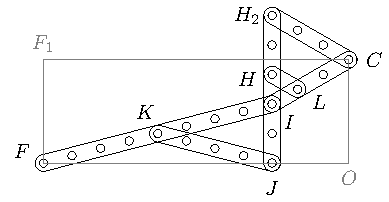
\includegraphics[scale=1]{9/cluster9b1}
\caption{Construction of distance $\overline{FC}=\sqrt{79 + 18\sqrt5}$}
\label{fig:cluster9b1}
\end{figure}

Figure \ref{fig:cluster9b1} show one of several ways to build the distance $\sqrt{79 + 18\sqrt5}$. 
Equilateral triangle $\triangle{FIZ}$ and isosceles $\triangle{IJK}$ share vertice $I$ and the base $\overline{JZ}$ which help to form rectangle $FXCY$ with base $\overline{FX}$ and height $\overline{FY}$ useful to calculate the diagonal $\overline{FC}$:
\begin{align}
\overline{FX} &= \overline{YJ} + \overline{JC}\nonumber\\
 &= \sqrt{\overline{FI}^2 - \left(\frac{\overline{IZ}}2\right)^2}
  + \sqrt{\overline{IC}^2 - \overline{IJ}^2}
  = \sqrt{3^2 - \left(\frac{3}2\right)^2} + \sqrt{8^2 - 2^2} 
  = \frac{3\sqrt3}2 + 2\sqrt{15} \nonumber\\
\overline{FY} &= \overline{JI} + \frac{\overline{IZ}}2
  = 2 + \frac{3}2 = \frac{7}2 \nonumber\\
\overline{FC} &= \sqrt{\overline{FX}^2 + \overline{FY}^2}
 = \sqrt{\left(\frac{3\sqrt3}2 + 2\sqrt{15}\right)^2 + \left(\frac{7}2\right)^2}
 = \sqrt{79 + 18\sqrt5} \quad\blacksquare
\end{align}

We use a smaller part of this construction, the five strips with vertices $F,G,H,I,J,K,C$, as a cluster to made rigid the consecutive strips $\overline{AB},\overline{BC}$ of the pentagon of side $9$ of figure \ref{fig:penta9b}.


\subsubsection{Rigid distance $\dfrac{\sqrt{334 + 90\sqrt5}}2$}

Our software found several options with five strips to build distance$\dfrac{\sqrt{334 + 90\sqrt5}}2$.

\begin{figure}[H]
\centering
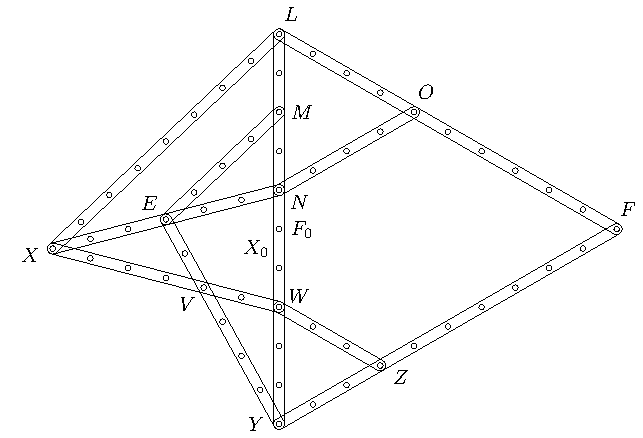
\includegraphics[scale=1]{9/cluster9b2}
\caption{Construction of distance $\overline{EF}=\dfrac{\sqrt{334 + 90\sqrt5}}2$}
\label{fig:cluster9b2}
\end{figure}

Figure \ref{fig:cluster9b2} show equilateral triangle $\triangle{FLY}$ and isoscelles triangle $\triangle{NXW}$ sharing strip $\overline{LY}$ which helps to calculate abscissas and ordinates of vertices $E,F$ to calculate distance $\overline{EF}$. Vertice $Y$ is located at the origin so:
\begin{align}
E_x &= - \left(\frac{\overline{NE}}{\overline{NX}}\right)\overline{XX_0}
 = -\frac{3}6\sqrt{\overline{NX}^2 - \overline{NX_0}^2}
 = -\frac{1}{2}\sqrt{6^2 - \left(\frac{3}2\right)^2} = -\frac{3\sqrt{15}}4 \\
E_y &= \overline{YN} - \left(\frac{\overline{NE}}{\overline{NX}}\right)\overline{NX_0}
 = 6 - \left(\frac{3}6\right)\left(\frac{3}2\right) = \frac{21}4\\
F_x &= \overline{F_0F} = \sqrt{\overline{YF}^2 - \overline{YF_0}^2}
 = \sqrt{10^2 - 5^2} = 5\sqrt3\\
F_y &= \overline{YF_0} = 5\\
\overline{EF} &= \sqrt{(E_x - F_x)^2 + (E_y - F_y)^2}
 = \sqrt{\left(-\frac{3\sqrt{15}}{4} -5\sqrt3 \right)^2 + \left(\frac{21}4 - 5\right)^2}
 = \frac{\sqrt{334+90\sqrt5}}2 \quad\blacksquare
\end{align}
We form a cluster from the last construction to be applied in the pentagon of side $9$. We choose the five strips with vertices $E,N,M,L,O,F$. Is easy to prove strip $\overline{EM}$ is correct in the cluster comparing equal cosines at vertice $Y$ for triangles $\triangle{YVW},\triangle{YEN},\triangle{YEM}$ using the law of cosines for each triangle.


% 10

\section{Pentagon of size 10}

\subsection{Size 10 with 10 internal strips $build(7:10)$}

\begin{figure}[H]
 \centering
 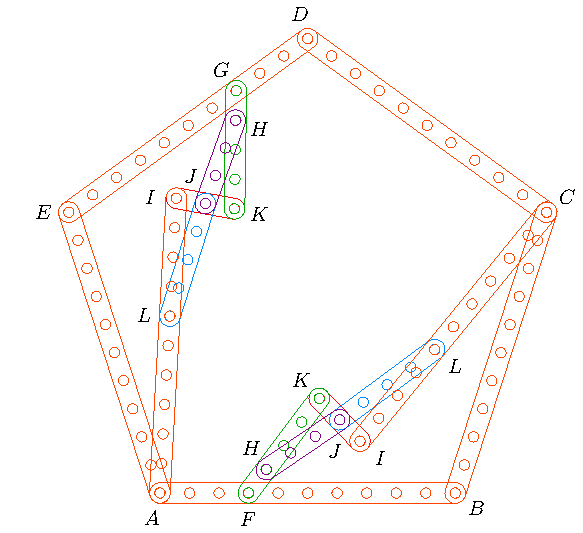
\includegraphics[scale=0.9]{10/penta10a}
 \caption{Pentagon size 10 with 10 interal strips. $\overline{FB}:\overline{BC} = 7:10$ and $\overline{CF} = \sqrt{114 + 35\sqrt5}$.}
 \label{fig:penta10a}
\end{figure}

Figure \ref{fig:penta10a} show a rigid regular pentagon $A,B,C,D,E$ of size 10. We calculate a diagonal joining two consecutive sides relative primes to have something exclusive to the size 10, we choose $\overline{BF}:\overline{BC} = 7:10$. With the law of cosines we calculate $\overline{CF}$.
We calculate the angle $\angle{CFB}$ for the drawing:
\begin{align}
\overline{CF}^2 &= \overline{BC}^2 + \overline{BF}^2
 - 2(\overline{BC})(\overline{BF})\cos\left(\frac{3\pi}5\right) \nonumber\\
 &= 10^2 + 7^2 - 2(10)(7)\left(\frac{1-\sqrt5}4\right) = 114 + 35\sqrt5 \nonumber\\
\overline{CF} &= \sqrt{114 + 35\sqrt5} \\
\cos(\angle{CFB}) &= \frac{\overline{CF}^2 + \overline{BF}^2 - \overline{BC}^2}
 {2(\overline{CF})(\overline{BF})}%\nonumber\\
 = \frac{114+35\sqrt5 + 7^2 - 10^2}{2(\sqrt{114 + 35\sqrt5})(7)}
  = \frac{9+5\sqrt5}{2\sqrt{114+35\sqrt5}}
\end{align}

\subsubsection{Rigid distance $\sqrt{114+35\sqrt5}$}

\begin{figure}[H]
 \centering
 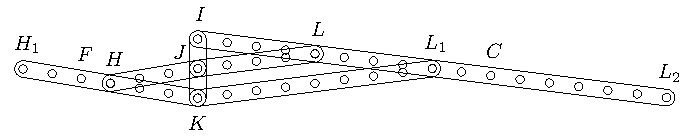
\includegraphics[scale=1.3]{10/cluster10a}
 \caption{Construction of distance $\overline{CF} = \sqrt{114+35\sqrt5}$}
 \label{fig:cluster10a}
\end{figure}

Our software found several solutions for this distance using five strips, and we choose one narrow enough to fit inside the pentagon.
\\\\
Figure \ref{fig:cluster10a} shows how to prove the cluster selected is correct. In the figure we have two isoscelles triangles $\triangle{IKL_1}$ and $\triangle{JKH}$. The sides $IL_1$ and $KH$ are extended to double the original size to the vertices $L_2$ and $H_1$ building two right angles $\angle{IKL_2}$ and $\angle{KJH_1}$. The right triangles permit the calculation of the abscissas and ordinates of vertices $C$ and $F$ to calculate their distance.
\\\\
From the figure we calculate $\overline{KL_2}$ and $\overline{JH_1}$ from their respective right triangles:
\begin{align}
\overline{KL_2} = \sqrt{(\overline{IL_2})^2 - (IK)^2} = \sqrt{16^2 - 2^2} = 6\sqrt7\\
\overline{JH_1} = \sqrt{(\overline{KH_1})^2 - (KJ)^2} = \sqrt{6^2 - 1^2} = \sqrt{35}
\end{align}

Assuming vertice $K$ is at the origin we can calculate the abscissas $C_x,F_x$ and ordinates $C_y,F_y$ of vertices $C$ and $F$ using as factors $c = \dfrac{\overline{IC}}{\overline{IL_2}} = \dfrac{10}{16} = \dfrac{5}8$ and $f = \dfrac{\overline{KF}}{\overline{KH1}}=\dfrac{4}6 = \dfrac{2}3$:
\begin{align}
C_x &= +c(\overline{KL_2}) = \frac{5}{8}(6\sqrt7) = \frac{15}{4}\sqrt7\\
F_x &= -f(\overline{JH_1}) = -\frac{2}{3}\sqrt{35}\\
C_y &= +(\overline{KI}) - c(\overline{KI}) = 2 - \frac{5}{8}(2) = \frac{3}4\\
F_y &= +f(\overline{KJ}) = \frac{2}{3}(1) = \frac{2}3
\end{align}

Finally we calculate the distance $\overline{CF}$:
\begin{align}
\overline{CF} &= \sqrt{(C_x - F_x)^2 + (C_y - F_y)^2}\nonumber\\
 &= \sqrt{\left(\frac{15}{4}\sqrt7 + \frac{2}{3}\sqrt{35}\right)^2
 + \left(\frac{3}4 - \frac{2}3\right)^2} %\nonumber\\
 %&= \sqrt{\dfrac{1575}{16} + 35\sqrt5 + \dfrac{140}9 + \dfrac{1}{144}} 
 = \sqrt{114+35\sqrt5} \quad\blacksquare
\end{align}
A minimal part with five strips of the construction of figure \ref{fig:cluster10a} including only vertices $F,H,I,J,K,L,C$ is used twice to make rigid the pentagon of side 10 as show in figure \ref{fig:penta10a}.

\subsection{Size 10 with 10 internal strips $build(8:10)$}

\begin{figure}[H]
 \centering
 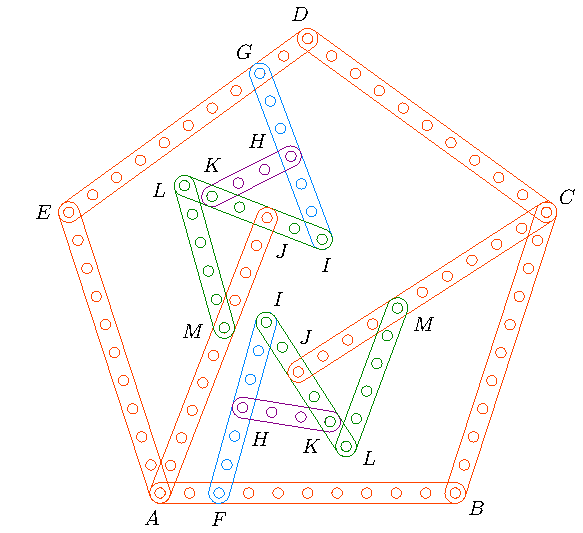
\includegraphics[scale=0.9]{10/penta10b}
 \caption{Pentagon size 10 with 10 internal strips. $\overline{FB}:\overline{BC} = 8:10$ and $\overline{CF} = 2\sqrt{31 + 10\sqrt5}$.}
 \label{fig:penta10b}
\end{figure}

Figure \ref{fig:penta10b} show a rigid regular pentagon $A,B,C,D,E$ of size 10. We include here the relation $\overline{FB}:\overline{BC} = 8:10$ since the relation $4:5$ for pentagon size $5$ gave clusters that can't fit inside such pentagon. With the law of cosines we calculate $\overline{CF}$ and
the angle $\angle{CFB}$ for the drawing:
\begin{align}
\overline{CF}^2 &= \overline{BC}^2 + \overline{BF}^2
 - 2(\overline{BC})(\overline{BF})\cos\left(\frac{3\pi}5\right) \nonumber\\
 &= 10^2 + 8^2 - 2(10)(8)\left(\frac{1-\sqrt5}4\right) = 124 + 40\sqrt5 \nonumber\\
\overline{CF} &= 2\sqrt{31 + 10\sqrt5} \\
\cos(\angle{CFB}) &= \frac{\overline{CF}^2 + \overline{BF}^2 - \overline{BC}^2}
 {2(\overline{CF})(\overline{BF})}%\nonumber\\
 = \frac{124+40\sqrt5 + 8^2 - 10^2}{2(2\sqrt{31 + 10\sqrt5})(8)}
  = \frac{11 + 5\sqrt5}{4\sqrt{31+10\sqrt5}}
\end{align}

\subsubsection{Rigid distance $2\sqrt{31 + 10\sqrt5}$}

One solution from our software is shown in figure as cluster $FHIJKLM$. Assume vertex $J$ is at the origin, vertice $I$ at $(-2,0)$ and vertice $K$ at $(+2,0)$. Since triangle $\triangle{IKH}$ is isoscelles and $\overline{IF}$ is the double of $\overline{IH}$ then angle $\angle{FKI} = \frac{\pi}2$ and we can calculate the abscissa and the ordinate of vertice $F$:
\begin{align}
F_x &= \overline{JK} = 2\\
F_y &= -\sqrt{(\overline{IF})^2 - (\overline{IK})^2} = -\sqrt{6^2 - 4^2} = -2\sqrt5
\end{align}

Since we have the Pythagorean triangle $\triangle{JLM}$ is easy to note that the abscissa and ordinate of vertice $C$ are $C_x = 0$ and $C_y = \overline{JC} = 10$, so finally we have:
\begin{align}
\overline{CF} &= \sqrt{(F_x - C_x)^2 + (F_y - C_y)^2} \nonumber\\
 &= \sqrt{(2 - 0)^2 + (-2\sqrt5 - 10)^2 } = 2\sqrt{31 + 10\sqrt5} \quad\blacksquare
\end{align}

% 11

\section{Pentagon of size 11}

\subsection{Size 11 with 10 internal strips $build(8:11)$}

\begin{figure}[h]
 \centering
 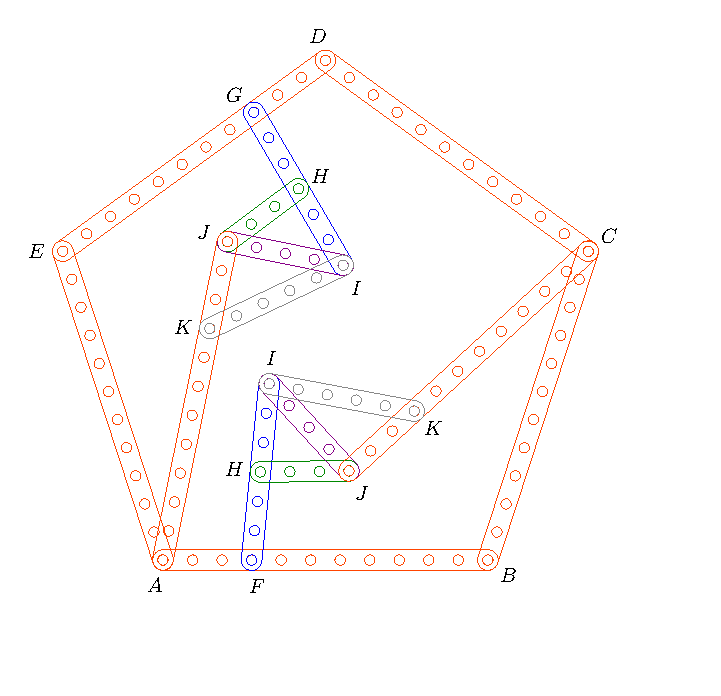
\includegraphics[scale=0.85]{11/penta11a}
 \caption{Pentagon size 11 with 10 internal strips. $\overline{FB}:\overline{BC} = 8:11$ and $\overline{CF} = 11 + 2\sqrt5$.}
 \label{fig:penta11a}
\end{figure}

Figure \ref{fig:penta11a} show a rigid regular pentagon $A,B,C,D,E$ of size 11. Our software found this is the smallest pentagon having a consecutive sides diagonal distance of the form $\dfrac{z_2 + z_3\sqrt5}{z_1}$ instead of the nested form $\dfrac{z_2\sqrt{z_3+z_4\sqrt5}}{z_1}$ where $z_i$ are integers. The mentioned diagonal is the distance $\overline{CF}$ in the figure which can be calculated with the law of cosines knowing angle $\angle{CBF} = \dfrac{3\pi}5$ and denesting the result. We calculate the angle $\angle{CFB}$ for the drawing:
\begin{align}
\overline{CF}^2 &= \overline{BC}^2 + \overline{BF}^2 
 - 2(\overline{BC})(\overline{BF})\cos\left(\dfrac{3\pi}5\right) \nonumber\\
 &= 11^2 + 8^2 - 2(11)(8)\left(\frac{1-\sqrt5}4\right) = 141 + 44\sqrt5 \nonumber\\
\overline{CF} &= \sqrt{141 + 44\sqrt5} \nonumber\\
 &= 11 + 2\sqrt5 \\
%
\cos(\angle{CFB}) &= \frac{\overline{CF}^2 + \overline{BF}^2 - \overline{BC}^2}
 {2(\overline{CF})(\overline{BF})}%\nonumber\\
 = \frac{141+44\sqrt5 + 8^2 - 11^2}{2(11+2\sqrt5)(8)}
  = \frac{21+11\sqrt5}{44+8\sqrt5} = \frac{121+79\sqrt5}{404}
\end{align}

\subsubsection{Rigid istance $11+2\sqrt{5}$}

A five strips cluster can create a rigid distance like $11 + 2\sqrt{5}$. In the figure, three strips $\overline{FI} = 2\overline{HJ}, \overline{FI} > \overline{IJ}$ builds a right angle $\angle{FJI} = \frac{\pi}2$, since triangle $\triangle{IJH}$ is isosceles ($\overline{FH} = \overline{HI} = \overline{JH}$). These three strips also build a distance $\overline{FJ} = \sqrt{\overline{FI}^2 - \overline{IJ}^2} = \sqrt{6^2 - 4^2} = 2\sqrt5$. Now we attach strip $\overline{CJ}$ making a second right triangle $\angle{CJI} = \frac{\pi}2$ using strip $\overline{IK}=5$ as pythagorean diagonal ($\overline{JK}=3, \overline{IJ}=4$). We have two right triangles at vertice $J$ so vertices $F,J,C$ are collinear, so we can calculate the distance $\overline{FC} = \overline{CJ} + \overline{JF} = 11 + 2\sqrt5 \quad\blacksquare$. 

We repeat the five-strips cluster between vertices $A,G$ preventing strips overlaps. Since the clusters are rigid we formed two rigid triangles $\triangle{ABC}, \triangle{DEA}$ so the pentagon is rigid.
\\\\
The software found the next pentagon of this type is a lot bigger: $\overline{BC}=246, \overline{BF}=70, \overline{CF}=41+105\sqrt5$.



% 12

\section{Pentagons of size 12}

\subsection{Size 12 with 4 internal strips $build(0:12:3:4)$}

Our sofware found that side $12$ is the smallest pentagon that can be made rigid with a rhoumbus and two strips as diagonals so need only 4 strips as diagonals.

\begin{figure}[h]
 \centering
 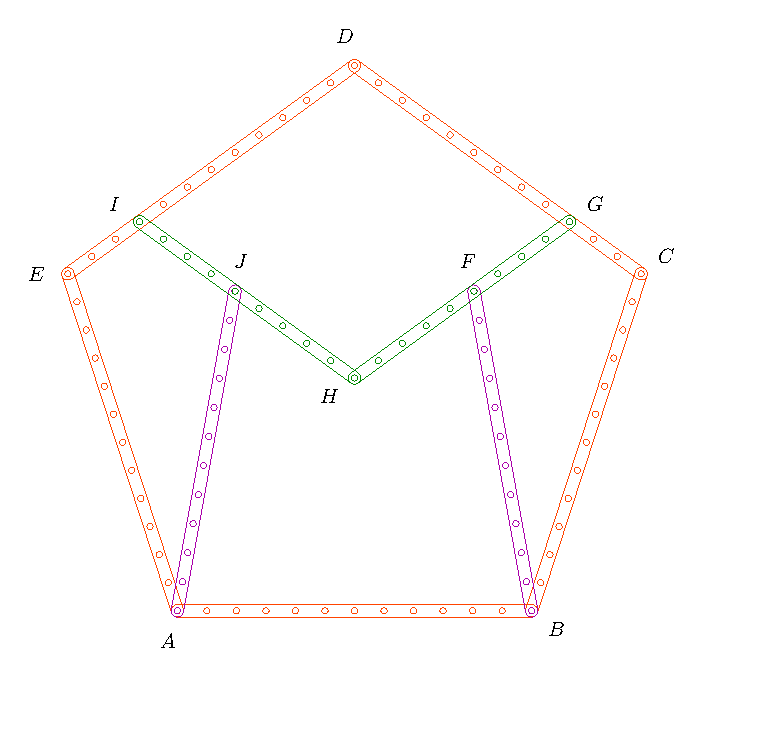
\includegraphics[scale=0.8]{12/penta12a}
 \caption{Pentagon size 12 with 4 internal strips. $\overline{AA}:\overline{AE}:\overline{EI}:\overline{IJ} = 0:12:3:4$ and $\overline{AJ}=11$.}
 \label{fig:penta12a}
\end{figure}

Figure \ref{fig:penta12a} show a regular pentagon $A,B,C,D,E$ of side 12 with a rhombus $D,I,H,G$ of side $9$. We prove strips $AJ,BF$ are correct. First we calculate the abscissas going through vertices $A,E,I,J$ substracting when we move to the left and adding when we move to the right:
\begin{align}
AJ_x &= AE_x + EI_x + IJ_x\nonumber\\
 &= -\overline{AE}\cos\left(\frac{2\pi}5\right)
 + \overline{EI}\cos\left(\frac{\pi}5\right) 
 + \overline{IJ}\cos\left(\frac{\pi}5\right)\nonumber\\
 &= -12\left(\frac{\sqrt5 - 1}4\right)
  +3\left(\frac{1+\sqrt5}4\right)
  +4\left(\frac{1+\sqrt5}4\right) 
  = \frac{19-5\sqrt5}4
\end{align}

Then we calculate the ordinates going to the same order of vertices adding when we go up and substracting when we go down:
\begin{align}
AJ_y &= -AE_y + EI_y + IJ_y\nonumber\\
 &= \overline{AE}\sin\left(\frac{2\pi}5\right)
 + \overline{EI}\sin\left(\frac{\pi}5\right) 
 - \overline{IJ}\sin\left(\frac{\pi}5\right)\nonumber\\
 &= 12\left(\frac{\sqrt{10+2\sqrt5}}4\right)
 + 3\left(\frac{\sqrt{10-2\sqrt5}}4\right)
 - 4\left(\frac{\sqrt{10-2\sqrt5}}4\right)%\nonumber\\
 %&= \frac{12\sqrt{10+2\sqrt5} - \sqrt{10-2\sqrt5}}4 
 = \frac{\sqrt{1450+190\sqrt5}}4
\end{align}
Finally we calculate the distance $\overline{AJ}$ which coincides with strip size $11$:
\begin{align}
\overline{AJ} &= \sqrt{(AJ_x)^2 + (AJ_y)^2}\nonumber\\
 &= \sqrt{\left(\frac{19-5\sqrt5}4\right)^2 + \frac{1450+190\sqrt5}{16}}%\nonumber\\
 %&= \sqrt{\frac{486-190\sqrt5}{16} + \frac{1450+190\sqrt5}{16}} 
 = \sqrt{121} = 11 \quad\blacksquare
\end{align}

\subsection{Size 12 with 4 internal strips $build(4:12:0:3)$}

\begin{figure}[H]
 \centering
 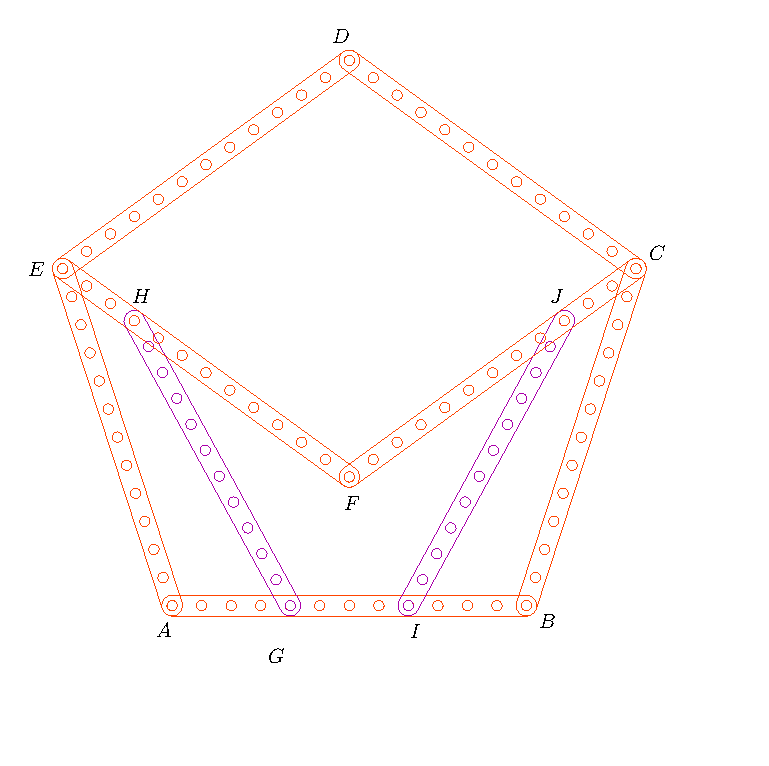
\includegraphics[scale=0.8]{12/penta12b}
 \caption{Pentagon size 12 with 4 internal strips. $\overline{GA}:\overline{AE}:\overline{EE}:\overline{EH} = 4:12:0:3$ and $\overline{GH}=11$.}
 \label{fig:penta12b}
\end{figure}

Figure \ref{fig:penta12b} show a regular pentagon $A,B,C,D,E$ of size 12 with a rhombus $D,I,H,G$ of size $12$. We prove strips $GH,IJ$ are correct. First we calculate the abscissas going through vertices $G,A,E,H$ substracting when we move to the left and adding when we move to the right:
\begin{align}
GH_x &= -GA_x - AE_x + EH_x\nonumber\\
 &= -\overline{GA} - \overline{AE}\cos\left(\frac{2\pi}5\right)
 +\overline{EH}\cos\left(\frac{\pi}5\right)\nonumber\\
 &= -4 - 12\left(\frac{\sqrt5 - 1}4\right) + 3\left(\frac{1+\sqrt5}4\right)
 = \frac{-1-9\sqrt5}4
\end{align}

Then we calculate the ordinates going to the same order of vertices adding when we go up and substracting when we go down:
\begin{align}
GH_y &= AG_y + AE_y - EH_y\nonumber\\
 &= 0 + \overline{AE}\sin\left(\frac{2\pi}5\right)
 - \overline{EH}\sin\left(\frac{\pi}5\right)\nonumber\\
 &= 12\left(\frac{\sqrt{10+2\sqrt5}}4\right)
 - 3\left(\frac{\sqrt{10-2\sqrt5}}4\right)%\nonumber\\
 %&= \frac{12\sqrt{10+2\sqrt5} -3\sqrt{10-2\sqrt5}}4 
 = \frac{\sqrt{1530-18\sqrt5}}4
\end{align}

Finally we calculate the distance $\overline{GH}$ which coincides with strip size $11$:
\begin{align}
\overline{GH} &= \sqrt{(GH_x)^2 + (GH_y)^2}\nonumber\\
 &= \sqrt{\left(\frac{-1-9\sqrt5}{4}\right)^2 + \frac{1530-18\sqrt5}{16}}%\nonumber\\
 %&= \sqrt{\frac{406+18\sqrt5}{16} + \frac{1530-18\sqrt5}{16}} 
 = \sqrt{121} = 11 \quad\blacksquare
\end{align}

\subsection{Size 12 with 6 internal strips $build(12:12)$}

\begin{figure}[h]
 \centering
 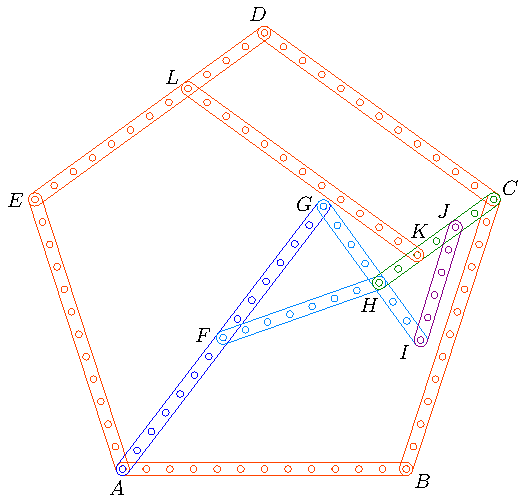
\includegraphics[scale=0.8]{12/penta12-6a}
 \caption{Pentagon size 12 with 6 internal strips. $\overline{AB}:\overline{BC} = 12:12$ and $\overline{AC} = 6 + 6\sqrt5$}.
 \label{fig:penta12-6a}
\end{figure}

Figure \ref{fig:penta12-6a} show a regular pentagon $A,B,C,D,E$ of side 12. We know the regular pentagon diagonal for size 12 is $\overline{AC} = 12\left(\dfrac{1+\sqrt5}2\right) = 6 + 6\sqrt5$. 

\subsubsection{Rigid distance $6 + 6\sqrt5$}

We show the five strips $\overline{GH},\overline{GI},\overline{HF},\overline{HC},\overline{IJ}$ make the diagonal rigid which makes rigid the angle $\angle{ABC}$ of the pentagon. We have an isoscelles triangle $\triangle{FGH}$ and $\overline{AG}$ is two times $\overline{FG}$ so we have a right angle $\angle{AHG} = \frac{\pi}2$ and we can calculate $\overline{AH} = \sqrt{(\overline{AG})^2 - (\overline{GH})^2} = \sqrt{14^2-4^2} = 6\sqrt5$. Now we have another right angle $\angle{IHC} = \frac{\pi}2$ because the Pythagoras triangle $\triangle{HIJ}$. Since $G,H,I$ are collinear then we have another right angle $\angle{GHC}=\frac{\pi}2$. Both right angles $\angle{AHG},\angle{CHG}$ guaranty vertices $A,H,C$ are collinear and we can calculate $\overline{AC} = \overline{AH} + \overline{HC} = 6 + 6\sqrt5$ $\blacksquare$.

Finally we add a sixth strip $\overline{KL}$ parallel to $\overline{CD}$ to make rigid the last three perimeter strips $\overline{CD},\overline{DE},\overline{EA}$ of the pentagon.

\subsection{Size 12 with 8 internal strips $build(6:12:3:6)$}

\begin{figure}[h]
 \centering
 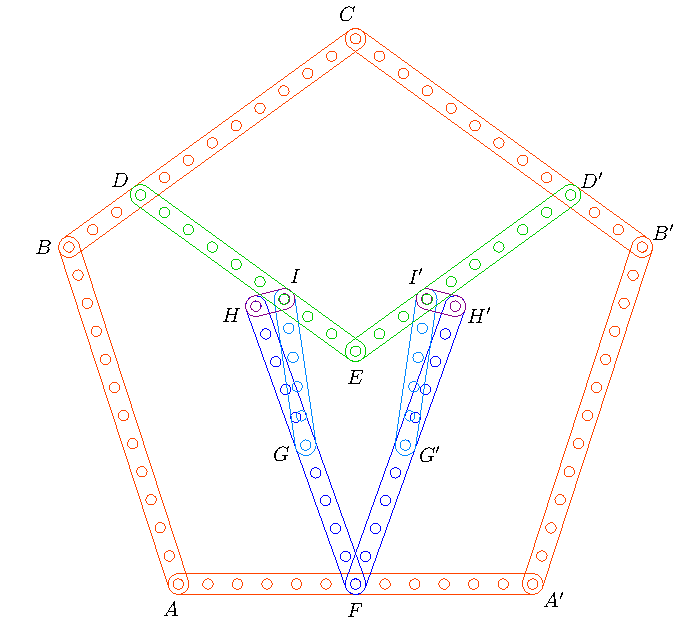
\includegraphics[scale=0.8]{12/penta12-8a}
 \caption{Pentagon size 12 with 8 internal strips. $\overline{FA}:\overline{AB}:\overline{BD}:\overline{DI} = 6:12:3:6$ and $\overline{FI} = 3\sqrt{11}$}.
 \label{fig:penta12-8a}
\end{figure}

Figure \ref{fig:penta12-8a} show a regular pentagon $AA'B'CBA$ of side 12.
First we calculate the distance $\overline{FI}$ using the abscissas and ordinates following the vertices $F,A,B,D,I$ for a regular pentagon angles $\alpha=\dfrac{3\pi}5, \beta=\dfrac{\pi}5$:
\begin{align}
FI_x &= -\overline{AF} - \overline{AB}\cos\alpha + (\overline{BD} + \overline{DI})\cos\beta\nonumber\\
 &= -6 + (12)\frac{1-\sqrt5}4 + (3+6)\frac{\sqrt5+1}4 = -\frac{3+3\sqrt5}4\\
FI_y &= \overline{AB}\sin\alpha + (\overline{BD}-\overline{DI})\sin\beta\nonumber\\
 &= (12)\frac{\sqrt{10+2\sqrt5}}4 + (3-6)\frac{\sqrt{10-2\sqrt5}}4
 = \frac{12\sqrt{10+2\sqrt5} - 3\sqrt{10-2\sqrt5}}4\\
\overline{FI} &= \sqrt{(FI_x)^2 + (FI_y)^2}\nonumber\\
 &= \frac{\sqrt{(-3-3\sqrt5)^2 + (12\sqrt{10+2\sqrt5} - 3\sqrt{10-2\sqrt5})^2}}4
 = \frac{\sqrt{1584}}4 = 3\sqrt{11}
\end{align}

\subsubsection{Rigid distance $3\sqrt{11}$}

Finally we calculate the distance $\overline{FI}$ made rigid by cluster $F,G,H,I$. We have an isoscelles triangle $\triangle{GHI}$ and $\overline{FH}=2\overline{GH}$ so we have a right triangle $\angle{FIH}=\frac{\pi}2$ so: \begin{align}
\overline{FI} &= \sqrt{(\overline{FH})^2 - (\overline{HI})^2}\nonumber\\
 &= \sqrt{10^2 - 1^2} = 3\sqrt{11}
\end{align}

\subsection{Size 12 with 10 internal strips $build(3:12:12)$}

\begin{figure}[H]
 \centering
 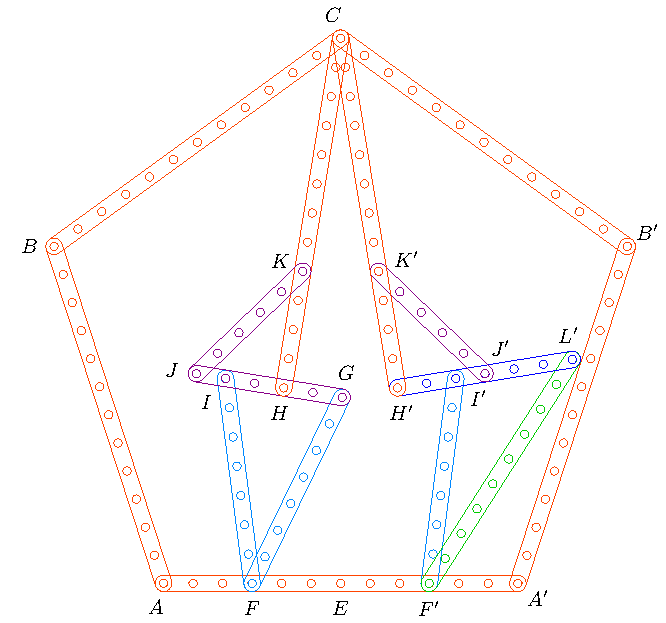
\includegraphics[scale=0.80]{12/penta12-10a}
 \caption{Pentagon size 12 with 10 internal strips.  $\overline{FA}:\overline{AB}:\overline{BC} = 3:12:12$ and $\overline{CF} = 12 + 3\sqrt5$.}
 \label{fig:penta12-10a}
\end{figure}

Figure \ref{fig:penta12-10a} show a regular pentagon $AA'B'CB$ of side 12. We know the regular pentagon height is $\dfrac{\sqrt{5+2\sqrt5}}2$ times the side. So here we have $\overline{CE} = 12\frac{\sqrt{5+2\sqrt5}}2 = 6\sqrt{5+2\sqrt5}$ and we can calculate $\overline{CF}$:
\begin{align}
\overline{CF} &= \sqrt{\overline{CE}^2 + \overline{EF}^2}\nonumber\\
 &= \sqrt{36(5+2\sqrt5) + 3^2} = 3\sqrt{21+8\sqrt5} \nonumber\\
 &= 3(4 + \sqrt5)
\end{align}

\subsubsection{Rigid distance $3(4 + \sqrt5)$}

After testing $\overline{AA'} \le 1800$ our software found that the last denesting is somehow special since other fractions $\dfrac{\overline{AF}}{\overline{AA'}} \neq \dfrac{1}4$ generated $\overline{CF}$s that can't be denested.

We have the Pythagorean triangle $\triangle{HJK}$ and the isoscelles $\triangle{FGI}$ so vertices $FHC$ are collinear. First we calculate $\overline{FH} = \sqrt{\overline{FG}^2 - \overline{GH}^2} = \sqrt{7^2 - 2^2} = 3\sqrt5$ and then $\overline{FC} = \overline{FH} + \overline{HC} = 3\sqrt{5} + 12$ matching last calculation. Finally we prove angle $\angle{F'H'L'} = \frac{\pi}2$ noting $\overline{F'H'} = \sqrt{(\overline{F'L'})^2 - (\overline{H'L'})^2} = \sqrt{9^2 - 6^2} = 3\sqrt5$ matching $\overline{FH}$ $\blacksquare$.




\end{document}